\chapter{Estructuras algebraicas}

Una estructura algebraica es una par $(G, *)$, en donde $G$ es un conjunto no vacío y $*$ es una operación aplicable a los elementos dicho conjunto. Podrían haber más operaciones aplicables, por ejemplo, sin son aplicables las operaciones $*$ y $\bdot$, la estructura algebraica sería $(G, *, \bdot)$.

En general, una estructura algebraica es una $n-tupla: (a_1, a_2, \dots, a_n)$, donde $a_1$ es un conjunto no vacío dado, y $\{ a_2, \dots, a_n \}$ es un conjunto de operaciones aplicables a los elementos del conjunto $a_1$.

Las estructuras algebraicas nos permiten estudiar y clasificar objetos matemáticos en función de sus propiedades algebraicas. Algunos ejemplos de estructuras algebraicas incluyen grupos, anillos y campos.

\section{Grupos}

\subsection{Axiomas de grupo} \label{sec:axiomas-grupo}
\vspace{2mm}
\begin{fmd-definition}[Grupo]
	Dado un conjunto $G$, no vacío, una operación binaria o función $*: G \times G \rightarrow G$, define en $G$ una \textit{estructura de grupo} $(G, *)$ si se cumplen las siguientes propiedades:
	\begin{enumerate}
		\item[\textbf{G1}:] \textbf{Asociatividad}: $\forall x, y, z \in G \implies (x*y)*z = x * (y*z)$
		\item[\textbf{G2}:] \textbf{Existencia del neutro}: $\exists \, e \in G \mid \forall x \in G \implies x*e = e*x = x$
		\item[\textbf{G3}:] \textbf{Existencia de inversos}: $\forall x \in G, \exists x' \in G \mid x * x' = x'*x = e$
	\end{enumerate}
\end{fmd-definition}

Por lo tanto, un grupo es una estructura algebraica que consta de:
\begin{enumerate}[label=\alph*)]
	\item Un conjunto no vacío;
	\item Una operación binaria (una función con dos argumentos);
	\item Tres propiedades.
\end{enumerate}

\begin{fmd-example}
	Conjunto: $\Z$; Operación binaria: suma $(+)$; Propiedades:
	\begin{enumerate}
		\item Asociatividad: $(3 + 4) + 2 = 3 + (4 + 2)$
		\item Neutro: el cero, $0 + 3 = 3 + 0 = 3$
		\item Inversos: $4 + (-4) = (-4) + 4 = 0$
	\end{enumerate}
	En general: $\forall x, y, z \in \Z$
	\begin{enumerate}
		\item Asociatividad: $(x + y) + z = x + (y + z)$
		\item Neutro: $\exists \, 0 \in \Z / 0 + x = x + 0 = x$
		\item Inversos: $\forall x \in \Z , \exists \, (-x) \in \Z / x + (-x) = (-x) + x = 0$
	\end{enumerate}
	$(\Z, +)$ es un grupo.
\end{fmd-example}


\begin{fmd-definition}[Grupo abeliano]
	En caso de que $(G, *)$ cumpla además la propiedad conmutativa,
	
	\begin{enumerate}
		\item[\textbf{G4}:] \textbf{Conmutatividad}: $\forall x, y \in G \implies x*y = y*x$
	\end{enumerate}
	se llama grupo \textit{abeliano}\footnote{En homenaje al matemático noruego Niels Henrik Abel (1802-1829)} o \textit{conmutativo}.
\end{fmd-definition}


\textbf{Notas}:
\begin{enumerate}[label=\roman*)]
	\item Se dice que la operación $(*)$ es \textbf{cerrada} en el conjunto $G$, si $*: G \times G \rightarrow G$, en este caso, se dice que $(G, *)$ tiene una regla o \textbf{ley de composición interna}.
	
	\item Cuando $(G, *)$ es abeliana, es común llamar \textit{suma} o \textit{adición} a $*$, se dice que $*$ es aditiva, suele usarse el signo $+$, su inverso es el \textit{opuesto} y se indica $a' = -a$. Es común llamar \textit{cero} al neutro y denotarlo por $0$;
	\item Cuando $(G, *)$ es \textit{no abeliana} (o no lo sabemos), decimos que $*$ es multiplicativa, se usa ``$\bdot$'', su inverso se dice \textit{recíproco} y se utiliza $a' = a^{-1}$. Es usual llamar \textit{unidad} al neutro y denotarlo $1$.
	\item Cuando la cardinalidad\footnote{Ver sección \ref{sec:finitos}} $|G|$ es finita, decimos que el grupo es \textit{finito}.
	\item Dado un grupo $(G, *)$, $a\in G$ y $m \in \mathbb{Z}$, por convención $a^m = a*a* \cdots *a$, con $m$ factores si $m>0$, y $a^m = (a^{|m|})^{-1} =$ $\left(a*a* \cdots *a\right)' = a'*a'* \cdots *a'$ con $|m|$ factores $a'$ si $m<0$.
\end{enumerate}


\begin{fmd-definition}[Monoide]
	El par $(M, *)$, donde $M \ne \emptyset$, y $*$ es una función, es un monoide\footnote{Corresponde a la definición dada en \cite{rojoAlgebra8vaEd}.} si y solo si $*$ es una \textit{ley de composición interna} en $M$.
\end{fmd-definition}

\begin{definition}[Idempotencia] \label{def:idempotencia}
	Si $(G, *)$ es un monoide, es decir, una estructura algebraica con una ley de composición interna, se dice que $g \in G$ es idempotente si $g * g = g$
	
	La idempotencia es la propiedad de realizar una operación determinada varias veces y aún así obtener siempre el mismo resultado que se obtendría si se realizase una sola vez.
\end{definition}

\begin{fmd-definition}[Semigrupo]
	El par $(A, *)$, donde $A \ne \emptyset$, y $*$ es una función, es un semigrupo si y solo si $*$ es una ley interna y asociativa en $A$.
\end{fmd-definition}

\begin{proposition}[Unicidad del neutro]
	En cualquier grupo el neutro es único.
\end{proposition}
\begin{proof}
	Sae $(G, *)$ un grupo cualquiera. Supongamos $e, e' \in G$ dos elementos que cumplen la propiedad del neutro:
	\[ \begin{cases}
		\forall x \in G:& \quad e*x = x*e = x\\
		\forall x \in G:& \quad e'*x = x*e' = x
	\end{cases} \]
	Entonces:
	\[ \begin{cases}
		x = e':& \quad e*e' = e'*e = e'\\
		x = e:& \quad e'*e = e*e' = e
	\end{cases} \]
	por tanto:
	\[ e = e*e' = e' \]
\end{proof}


\begin{fmd-proposition}[Ley de corte o de cancelación]
	Sea $(G, *)$ un grupo. $\forall a, b, c \in G$ se cumple:
	
	\begin{enumerate}[label=\alph*)]
		\item Ley de corte por la izquierda: $a * b = a * c \implies b = c$
		\item Ley de corte por la derecha: $b*a = c*a \implies b = c$
	\end{enumerate}
	\begin{proof}
		Para demostrar a) basta con premultiplicar por el inverso $a'$ y en b) posmultiplicar.
	\end{proof}
\end{fmd-proposition}

Se dice que los elementos son \textbf{regulares} si se cumple la ley de corte.

\begin{proposition}[Unicidad del inverso]
	Para cualquier elemento $x \in G$ existe un inverso y es único.
	
	\begin{proof}
		Sea $(G, *)$ un grupo cualquiera. Supongamos $x', x'' \in G$ dos elementos que cumplen la propiedad del inverso:
		\[ \begin{cases}
			\forall x \in G:& \quad x*x' = x'*x = e\\
			\forall x \in G:& \quad x*x'' = x''*x = e
		\end{cases} \]
		Entonces:
		\[ x * x' = x * x'' \]
		
		por ley de cancelación: \[ x' = x'' \]
	\end{proof}
\end{proposition}

\begin{fmd-definition}[Orden de un grupo]
	Sea $(G, *)$ grupo. Llamamos orden de $G$ al número de elementos de $G$ (si $G$ es finito). Lo denotamos por $o(G) \coloneqq |G| = \mbox{card} (G) = \# (G)$
\end{fmd-definition}

Decimos que $G$ es de \textbf{orden par} u \textbf{orden impar} si $o(G)$ es par o impar respectivamente.

El grupo de orden 1, llamado \textbf{grupo trivial}, es el que consta de un solo elemento, el cual debe ser el neutro para cumplir con las propiedades de grupo. Es común utilizar tablas para representar las operaciones, denominadas \textbf{tablas de Cayley}\footnote{En homenaje al matemático británico Arthur Cayley (1821-1895)}.

Los conjuntos correspondientes a los grupos de orden 1, 2 y 3 son $\{ e \}$, $\{ e, a \}$, $\{e, a, b\}$. Sus respectivas tablas de Cayley se muestran en la tabla \ref{tab:cayley}:

\begin{table}[H]
	\centering
	\[ \begin{array}{c|c}
		* & e \\ \hline
		e & e
	\end{array} \qquad \quad \begin{array}{c|cc}
		* & e & a \\ \hline
		e & e & a \\
		a & a & e
	\end{array} \qquad \quad \begin{array}{c|ccc}
		* & e & a & b \\ \hline
		e & e & a & b \\
		a & a & b & e \\
		b & b & e & a
	\end{array}\]
	\caption{Tablas de Cayley para grupos de orden 1, 2 y 3.}
	\label{tab:cayley}
\end{table}
\begin{itemize}
	\item Notar que cada fila y columna contiene todos los elementos del grupo. No existen duplicados en ninguna fila ni columna.
	
	\item Estos grupos son abelianos ya que las tablas son simétricas respecto de la diagonal principal.
	\item Notar la similitud con las operaciones entre números enteros, si convertimos $* \rightarrow +, e \rightarrow 0, a \rightarrow 1, b \rightarrow 2$, que se muestran en la tabla \ref{tab:cayley2}, en este caso se dice que el grupo $(G, *)$ es \textbf{isomorfo} con su correspondiente $(\Z_n, +)$. Más adelante se verán estos conceptos con más detalle.
\end{itemize}

\begin{table}[H]
	\centering
	\[ \begin{array}{c|c}
		+ & 0 \\ \hline
		0 & 0
	\end{array} \qquad \quad \begin{array}{c|cc}
		+ & 0 & 1 \\ \hline
		0 & 0 & 1 \\
		1 & 1 & 0
	\end{array} \qquad \quad \begin{array}{c|ccc}
		+ & 0 & 1 & 2 \\ \hline
		0 & 0 & 1 & 2 \\
		1 & 1 & 2 & 0 \\
		2 & 2 & 0 & 1
	\end{array}\]
	\caption{Tablas de Cayley para enteros módulo 1, 2 y 3.}
	\label{tab:cayley2}
\end{table}

\textbf{Tarea}: Realizar las tablas de Cayley para grupos de orden 4.

\begin{fmd-example}[Grupo de Klein]
	El grupo de Klein\footnote{En honor al matemático alemán Felix Klein (1849-1925).} es abeliano con 4 elementos, en el cual cada elemento es su propio inverso (\textit{propiedad involutiva}), y componiendo cualesquiera dos de ellos, a excepción del neutro, produce el tercero, es decir:
	\[ V = \{ e, a, b, c \}; \quad a^2 = b^2 = (ab)^2 = c^2 = e \]
	\vspace{-15mm}
	\begin{table}[H]
		\centering
		\[ \begin{array}{c|cccc}
			\ast & e & a & b & c \\ \hline
			e & e & a & b & c \\
			a & a & e & c & b \\
			b & b & c & e & a\\
			c & c & b & a & e
		\end{array}\]
		\caption{Tabla de Cayley para el grupo de Klein.}
		\label{tab:Klein}
	\end{table}
\end{fmd-example}

\subsection{Grupos de números}

\textbf{Sistemas numéricos}.

Veamos el concepto de grupo para los \textit{sistemas numéricos} $\N, \Z, \Q, \R, \C$ y las operaciones usuales de suma $(+)$ y multiplicación $(\bdot)$.

En la fig. \ref{fig:sisnum} se representan gráficamente. Se observa que: $\N \subset \Z \subset \Q \subset \R \subset \C$.

\begin{figure}[h]
	\centering
	\includestandalone[scale=1.2]{resources/ltx/rectaN}
	\caption{Representación gráfica de los sistemas numéricos.}
	\label{fig:sisnum}
\end{figure}

\begin{table}[h]
	\centering
	\begin{tabular}{|l|c|c|c|c|c|}
		\hline
		& $(\N, +)$ & $(\Z, +)$ & $(\Q, +)$ & $(\R, +)$ & $(\C, +)$ \\
		& $(\N, \cdot)$ & $(\Z, \cdot)$ & $(\Q^{*}, \cdot)$ & $(\R^{*}, \cdot)$ & $(\C^{*}, \cdot)$ \\ \hline
		Asociativa & \cmark & \cmark & \cmark  & \cmark &  \cmark \\
		& \cmark & \cmark & \cmark  & \cmark  &  \cmark \\ \hline
		Neutro & 0 & 0 & 0  & 0 & 0 \\
		& 1 & 1 & 1  & 1  &  1 \\ \hline
		Inversos & \xmark & \cmark & \cmark  & \cmark & \cmark \\
		& \xmark & \xmark & \cmark  & \cmark & \cmark \\ \hline
	\end{tabular}
	\caption{Comprobación de las propiedades de Grupo para sistemas numéricos. Los conjuntos con $*$ indican que se excluye el cero. Los 7 grupos que comprueban las tres propiedades, además, son \textit{abelianos}.}
\end{table}
Notar que, a partir de $(\Z, \bdot)$ se deduce que restringiendo al par $\left(\{ -1, 1 \}, \bdot \right)$, este cumple las propiedades de grupo.


\subsection{Grupos de matrices} \label{sec:matrices}

Consideremos $\mathbf{M}_{m\times n}(\R)$, el conjunto de todas las matrices $m \times n$ con $m, n \in \N$ y elementos reales, el conjunto también puede ser representado por $\R^{m \times n}$.

\begin{equation}
	\mathbf{M}_{m \times n}(\R) = \left\{ \begin{bmatrix}
		a_{11} & \cdots & a_{1n}\\
		\vdots & \ddots & \vdots\\
		a_{m1} & \cdots & a_{mn}
	\end{bmatrix} | \, a_{ij} \in \R \right\}
	\label{eq:matrices}
\end{equation}

\subsubsection{Suma de matrices}

Dadas las matrices $A = (a_{ij})$ y $B = (b_{ij})$, se define la suma: $S = A + B = (s_{ij})$ de modo que $s_{ij} = a_{ij} + b_{ij}$, es decir, la matriz $S$ tiene como elementos la suma de los elementos correspondientes de $A$ y $B$.

Ejemplo:
\[ \begin{bmatrix}
	1 & 2\\
	3 & 4
\end{bmatrix} + \begin{bmatrix}
	5 & 6\\
	7 & 8
\end{bmatrix} = \begin{bmatrix}
	6 & 8\\
	10 & 12
\end{bmatrix} \]

Notar que la suma elemento a elemento ocurre en $\R$, conforme a la definición dada en \eqref{eq:matrices}. Por lo tanto, probar que $(\mathbf{M}_{m\times n}(\R), +)$ es un grupo se reduce a probar que $(\R, +)$ es un grupo, lo cual ya fue analizado junto con los demás sistemas numéricos, y se vió que $(\R, +)$ es un grupo abeliano, con lo cual,

las matrices cuadradas con la operación suma, cumplen:
\begin{itemize}
	\item[G1] Asociatividad: $(A + B) + C = A + (B + C)$ \quad \cmark 
	\item[G2] Neutro: $e_{2\times 3} = \begin{bmatrix} 0 & 0 & 0\\0 & 0 & 0 \end{bmatrix}$;
	$e_{m \times n} = \begin{bmatrix} 0 & \cdots & 0\\ \vdots & \ddots & \vdots\\ 0 & \cdots & 0 \end{bmatrix}$; $a_{ij} = 0$ \quad \cmark 
	\item[G3] Inversos (opuestos):  $(a_{ij})' = (-a_{ij})$ \quad \cmark 
	\item[G4] Conmutatividad: $A + B = B + A$ \quad \cmark 
\end{itemize}
por tanto:

\begin{center}
	$\left( \mathbf{M}_{m \times n}(\R), + \right)$ es un grupo abeliano.
\end{center}

El producto indicado $m \times n$ se conoce como \textbf{orden de la matriz}, así se dice por ejemplo de $A_{2 \times 3}$ es una matriz de orden $2 \times 3$.

\subsubsection{Grupos de vectores}

Un caso especial de matrices son los vectores. Consideremos, el conjunto de vectores en $\R^n$:
\begin{equation}
	\mathbf{M}_{1 \times n}(\R) = \left\{ \begin{bmatrix}
		a_1 \\ \vdots \\ a_n \end{bmatrix} | \, a_{i} \in \R \right\}
	\label{eq:vectores} = \R^n = \underbrace{\R \times \cdots \times \R}_{n \; veces}
\end{equation}

con la operación usual de suma.

Vectores con la operación suma. $\forall u, v, w \in \R^n$ se cumple:
\begin{itemize}
	\item[G1] Asociatividad: $(u + v) + w = u + (v + w)$ \quad \cmark 
	\item[G1] Neutro: $e_2 = \begin{bmatrix} 0 \\ 0 \end{bmatrix}$; $e_n = \begin{bmatrix} 0 \\ \vdots \\ 0 \end{bmatrix}$, $a_i = 0$ \quad \cmark 
	\item[G1] Inversos (opuestos): $u' = -u$ \quad \cmark 
	\item[G1] Conmutatividad: $u + v = v + u$ \quad \cmark 
\end{itemize}

\begin{center}
	$(\R^n, +)$ es un grupo abeliano.
\end{center}

Los vectores en $\R^2$ se representan en la fig. \ref{fig:grupoR2}:

\begin{figure}[h]
	\centering
	\includestandalone[]{resources/ltx/grupoR2}
	\caption{$(\R^2, +)$ es un grupo abeliano}
	\label{fig:grupoR2}
\end{figure}

\begin{enumerate}[label=\roman*)]
	\item Neutro: $(0,0)$
	\item Inverso de $u = (u_1, u_2)$ es $-u = (-u_1, -u_2)$.
\end{enumerate}

\subsubsection{Producto de matrices}

Dadas las matrices $A = (a_{ik}) \in \mathbf{M}_{m\times n}$ y $B = (b_{kj}) \in \mathbf{M}_{n\times r}$,

\begin{equation}
	A \cdot B = 
	\begin{bmatrix}
		a_{11} & \cdots & a_{1n}\\
		\vdots & \ddots & \vdots\\
		a_{m1} & \cdots & a_{mn}
	\end{bmatrix} \cdot \begin{bmatrix}
		b_{11} & \cdots & b_{1r}\\
		\vdots & \ddots & \vdots\\
		b_{n1} & \cdots & b_{nr}
	\end{bmatrix} = \begin{bmatrix}
		c_{11} & \cdots & c_{1r}\\
		\vdots & \ddots & \vdots\\
		c_{m1} & \cdots & c_{mr}
	\end{bmatrix} = C
\end{equation}
donde:

\begin{equation}
	c_{ij} = \sum_{k=1}^{n} a_{ik} b_{kj}
	\label{eq:cij}
\end{equation}
es, por definición, el producto de matrices.

Ejemplo:

\[ \begin{bmatrix}
	1 & 2 & 3\\
	-1 & 0 & 1
\end{bmatrix} \cdot \begin{bmatrix}
	4 \\ 5 \\ 1
\end{bmatrix} = \begin{bmatrix}
	17 \\ -3
\end{bmatrix} \]

\textbf{Notas}:

\begin{enumerate}[label=\roman*)]
	\item La operación es $\bdot : \textbf{M}_{m \times n} \times \mathbf{M}_{n \times r} \rightarrow \mathbf{M}_{m \times r}$, es decir, $(A, B) \rightarrow C$. El número de columnas de $A$ debe ser igual al número de filas de $B$ para que se realizable el producto. La matriz $C$ es de orden igual al número de filas de $A$ por el número de columnas de $B$.
	
	\item Las matrices de orden $m\times n$ con $m \ne n$ son llamadas \textbf{matrices rectangulares} y cuando $m = n$ se dice que son \textbf{cuadradas}.
	
	\item El producto de matrices es asociativo, es decir: \[(A_{m\times n} \cdot B_{n \times r}) \cdot C_{r \times s} = A_{m \times n} \cdot (B_{n \times r} \cdot C_{r \times s})\] Como puede comprobarse de la definición.
	
	\item Las matrices rectangulares con la operación de multiplicación definida en \eqref{eq:cij} no forman un grupo, pues la operación no es \textbf{cerrada}, es decir, en general las matrices $A, B, C$, con $C = AB$ no son del mismo orden, en otras palabras, no son del mismo conjunto, de donde no se cumple la condición $\bdot: G \times G \rightarrow G$, dada en la definición de grupo.
\end{enumerate}

Consideremos solo matrices cuadradas $\mathbf{M}_{n \times n}(\R) = \mathbf{M}_n(\R)$, en este caso, la operación de multiplicación $(\cdot)$ es cerrada, esto es:

\[ \bdot: \mathbf{M}_n \times \mathbf{M}_n \rightarrow \mathbf{M}_n\]

\begin{itemize}
	\item[G1:] Asociatividad: $(AB)C = A(BC)$ \quad \cmark
	\item[G2:] Elemento neutro: \quad \cmark
	\[I_n = \begin{bmatrix}
		1 & \cdots & 0\\
		\vdots & \ddots & \vdots\\
		0 & \cdots & 1 
	\end{bmatrix}; a_{ij} = \delta_{ij} = \begin{cases} 1 & \mbox{ si } i = j;\\ 0 & \mbox{ si } i \ne j \end{cases} \] $I_n$ es la matriz identidad de orden $n$; $\delta_{ij}$ se conoce como delta de Kronecker\footnote{En homenaje al matemático alemán Leopold Kronecker (1823-1891).}.
	\item[G3:] Inversos \quad \xmark
	
	No toda matriz $A \in \mathbf{M}_n$ tiene inversa, como se verá más adelante en el curso.
\end{itemize}

de donde, en general las matrices cuadradas de orden $n$ con la operación de multiplicación no son un grupo, se cumple que:

\begin{center}
	$(\mathbf{M}_n(\R), \bdot)$ es un semigrupo con elemento neutro.
\end{center}

Se llaman \textbf{matrices invertibles} aquellas que admiten inversa. La inversa de $A$ se denota como $A^{-1}$. Esto nos lleva a la definición siguiente:

\begin{fmd-definition}[Grupo General Lineal]
	
	Dado el conjunto de matrices cuadradas invertibles con entradas en $\R$:
	\[ GL_n(\R) = \left\{ A \in \mathbf{M}_n(\R) \mid \exists A^{-1} \right\} \subset \mathbf{M}_n(\R) \]
	y la operación de multiplicación de matrices $(\bdot)$.
	
	$(GL_n(\R), \bdot)$ se llama \textit{grupo general lineal}.
\end{fmd-definition}

Notar que $(GL_n(\R), \bdot)$ es efectivamente un grupo.

Se verá más adelante en el curso que el determinante de matrices invertibles es distinto de cero. Incorporando este concepto de determinante definimos otro grupo más pequeño que el anterior.

\begin{fmd-definition}[Grupo Especial Lineal]
	
	El conjunto de matrices cuadradas invertibles con determinantes iguales a uno:
	\[ SL_n(\R) = \left\{ A \in \mathbf{M}_n(\R) \mid \det A = 1 \right\} \]
	
	con la operación de multiplicación matricial, $(SL_n(\R), \bdot)$ se llama \textit{grupo especial lineal}.
\end{fmd-definition}
Notar que:
\[ SL_n(\R) \subset GL_n(\R) \subset \mathbf{M}_n(\R)\]

\subsection{Homomorfismo de grupos} \label{sec:homogrupo}

\begin{fmd-definition}[Homomorfismo]
	Dados los grupos $(G, \ast)$ y $(H, \bdot)$, un homomorfismo de $G$ a $H$ es una función $\phi: G \rightarrow H \, / \,  \forall a, b \in G \implies \phi(a*b) = \phi(a) \bdot \phi(b)$.
\end{fmd-definition}
\begin{figure}[H]
	\centering
	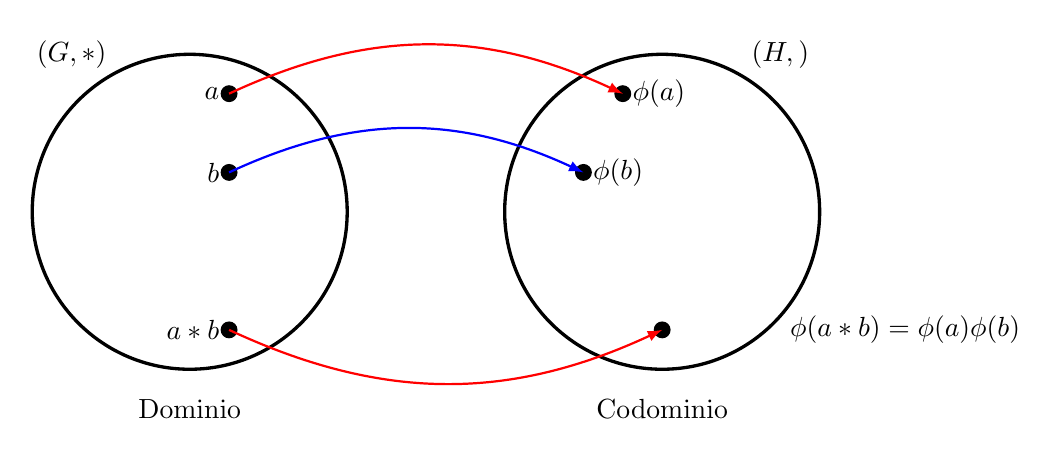
\begin{tikzpicture}[scale=1]
		% Coordenadas de puntos
		\coordinate (A0) at (0.5,1.5);
		\coordinate (Am1) at (.5,.5);
		\coordinate (A1) at (.5,-.5);
		\coordinate (A2) at (.5,-1.5);
		
		\coordinate (B0) at (5.5,1.5);
		\coordinate (B1) at (5,.5);
		\coordinate (B2) at (6,0);
		\coordinate (B3) at (6.5,-.75);
		\coordinate (B4) at (6,-1.5);
		
		% Circunferencias
		\node at (-1.5, 2) {$(G, *)$};
		\node at (7.5, 2) {$(H, \bdot)$};
		\draw[very thick] (0,0) circle (2);
		\draw[very thick] (6,0) circle (2);
		\node at (0, -2.5) {Dominio};
		\node at (6, -2.5) {Codominio};
		
		% Puntos
		\draw[fill] (A0) circle (1mm) node[left] {$a$};
		\draw[fill] (Am1) circle (1mm) node[left] {$b$};
		%			\draw[fill] (A1) circle (1mm) node[left] {$a*b$};
		\draw[fill] (A2) circle (1mm) node[left] {$a*b$};
		
		\draw[fill] (B0) circle (1mm) node[right] {$\phi(a)$};
		\draw[fill] (B1) circle (1mm) node[right] {$\phi(b)$};
		%			\draw[fill] (B2) circle (1mm) node[right] {2};
		%			\draw[fill] (B3) circle (1mm) node[right] {3};
		\draw[fill] (B4) circle (1mm) node[right, xshift=15mm] {$\phi(a*b) = \phi(a) \bdot \phi(b)$};
		
		% flechas
		\draw[red, thick, -latex] (A0) to [bend left = 25] (B0);
		\draw[blue, thick, -latex] (Am1) to [bend left = 25] (B1);
		%			\draw[blue, thick, -latex] (A1) to [bend left = -25] (B1);
		\draw[red, thick, -latex] (A2) to [bend left = -25] (B4);
	\end{tikzpicture}
	\caption{}
\end{figure}

\subsubsection{Propiedades}
\begin{enumerate}
	\item La imagen del neutro de $G$ es el neutro de $H$: $\phi(e_G) = e_H$.
	\[ \phi(a) = \phi(a*e_G) = \phi(a) \bdot \phi(e_G) = \phi(a) \bdot e_H \implies \phi(e_G) = e_H\]
	por elemento neutro en $(G, *)$, homomorfismo, elemento neutro en $(H, \bdot)$ y ley de cancelación.
	
	\item La imagen del inverso de todo elemento en $G$ es el inverso de su imagen en $H$: $\phi(a'_G) = a'_H$ o, en otra notación: $f(x^{-1}) = \left[f(x)\right]^{-1}$.
	
	\[ \forall x \in G: x * x^{-1} = e \implies f(x * x^{-1}) = f(e)\] por homomorfismo y propiedad 1:
	
	\[ f(x) \cdot f(x^{-1}) = e_H \implies f(x^{-1}) = \left[f(x)\right]^{-1} \]
	
	En un diagrama:
	\begin{figure}[H]
		\centering
		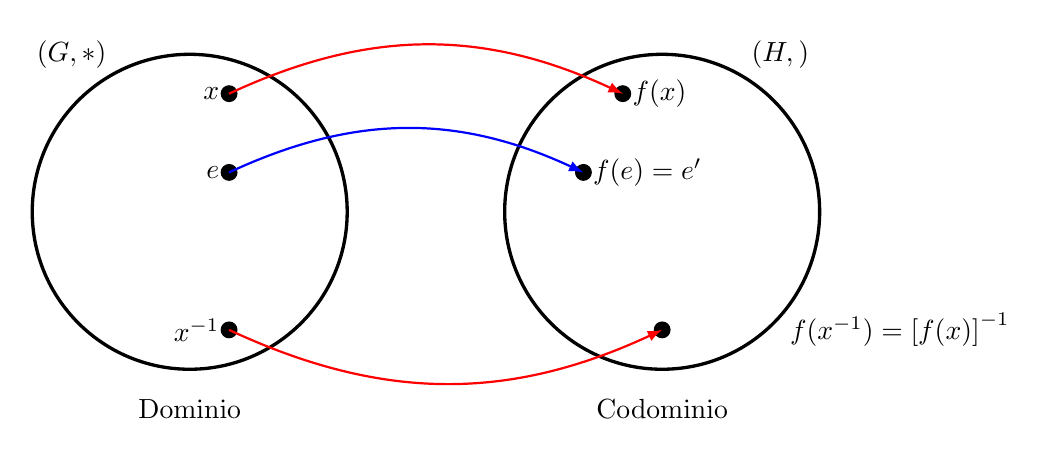
\begin{tikzpicture}[scale=1]
			% Coordenadas de puntos
			\coordinate (A0) at (0.5,1.5);
			\coordinate (Am1) at (.5,.5);
			\coordinate (A1) at (.5,-.5);
			\coordinate (A2) at (.5,-1.5);
			
			\coordinate (B0) at (5.5,1.5);
			\coordinate (B1) at (5,.5);
			\coordinate (B2) at (6,0);
			\coordinate (B3) at (6.5,-.75);
			\coordinate (B4) at (6,-1.5);
			
			% Circunferencias
			\node at (-1.5, 2) {$(G, *)$};
			\node at (7.5, 2) {$(H, \bdot)$};
			\draw[very thick] (0,0) circle (2);
			\draw[very thick] (6,0) circle (2);
			\node at (0, -2.5) {Dominio};
			\node at (6, -2.5) {Codominio};
			
			% Puntos
			\draw[fill] (A0) circle (1mm) node[left] {$x$};
			\draw[fill] (Am1) circle (1mm) node[left] {$e$};
			%			\draw[fill] (A1) circle (1mm) node[left] {$a*b$};
			\draw[fill] (A2) circle (1mm) node[left] {$x^{-1}$};
			
			\draw[fill] (B0) circle (1mm) node[right] {$f(x)$};
			\draw[fill] (B1) circle (1mm) node[right] {$f(e) = e'$};
			%	\draw[fill] (B2) circle (1mm) node[right] {2};
			%	\draw[fill] (B3) circle (1mm) node[right] {3};
			\draw[fill] (B4) circle (1mm) node[right, xshift=15mm] {$f(x^{-1}) = \left[f(x)\right]^{-1}$};
			
			% flechas
			\draw[red, thick, -latex] (A0) to [bend left = 25] (B0);
			\draw[blue, thick, -latex] (Am1) to [bend left = 25] (B1);
			%	\draw[blue, thick, -latex] (A1) to [bend left = -25] (B1);
			\draw[red, thick, -latex] (A2) to [bend left = -25] (B4);
		\end{tikzpicture}
	\end{figure}
\end{enumerate}

\textbf{Se dice que}:
\begin{enumerate}[label=\roman*)]
	\item $\phi$ es un \textit{mono}morfismo si es \textit{inyectiva};
	\item $\phi$ es un \textit{epi}morfismo si es \textit{sobreyectiva};
	\item $\phi$ es un \textit{iso}morfismo si es \textit{biyectiva};
	\item $\phi$ es un \textit{endo}morfismo si $G = H$;
	\item $\phi$ es un \textit{auto}morfismo si es un endomorfismo biyectivo.
\end{enumerate}
A veces deja de escribirse $*$ y $\bdot$ de modo que $\phi(ab) = \phi(a)\phi(b)$, sin embargo no debe perderse de vista que $ab$ ocurre en $G$ y $\phi(a)\phi(b)$ en $H$.

\begin{fmd-example}
	Dados $(\R, +)$ grupo de números reales para la adición y $(\R^+, \bdot)$ grupo de números reales positivos para la multiplicación. La aplicación $f: \R \rightarrow \R^+$ definida por $f(x) = 2^x$ es un homomorfismo ya que:
	\[ f(x + y) = 2^{x + y} = 2^x 2^y = f(x)f(y)\]
	En particular, $f$ es biyectiva, luego $(\R, +)$ y $(\R^+, \bdot)$ son isomorfos.
\end{fmd-example}

\begin{fmd-example}
	Para cualquier grupo $G$
	
	\begin{enumerate}
		\item El mapa nulo $\phi: G \rightarrow G$, dado por $\phi(x) = e_G, \forall x \in G$ y el mapa identidad $id: G \rightarrow G$, dado por $id(x) = x, \forall x \in G$, son endomorfismos.
		\item Si $a\in G$, el mapa $C_a: G \rightarrow G / C_a(b) = a^{-1}ba$ es un automorfismo. En efecto: \vspace{-1mm}
		\[ C_a(bc) = a^{-1}bca = a^{-1}b (aa^{-1}) ca = (a^{-1}ba)(a^{-1} ca) = C_a(b)C_a(c)\]
		es un homomorfismo, falta verificar que es invertible, su inversa es $C_{a^{-1}}: G \rightarrow G$ (verificar).
	\end{enumerate}
\end{fmd-example}

\begin{fmd-example}
	Dados $(\R^{+}, \times)$ grupo de números reales positivos con la operación de multiplicación y $(\R, +)$ grupo de números reales con la adición. Probar que la aplicación $f: \R^{+} \rightarrow \R$ definida por $f(x) = \ln x$ es un isomorfismo.
	
	Es un homomorfismo ya que $\ln(xy) = \ln x + \ln y$. Para probar que es un isomorfismo debemos mostrar que $f$ es biyectiva.
	
	\begin{enumerate}[label=\alph*)]
		\item $f$ es 1-1 si $f(x) = f(y) \implies x = y$
		\[ \ln x = \ln y \implies e^{\ln x} = e^{\ln y} \implies x = y \]
		$f$ es inyectiva.
		
		\item $f$ es sobreyectiva pues $\mbox{Im}(f) = \R$
		
		\begin{figure}[H]
			\centering
			\includestandalone[]{resources/ltx/log}
		\end{figure}
	\end{enumerate}
	De donde $f$ es biyectiva, por lo tanto los grupos mencionados son isomorfos bajo la función logaritmo natural.
\end{fmd-example}

\subsection{Grupos de simetrías}

\subsubsection{Grupos de funciones}
?`Cómo construimos grupos cuyos elementos sean funciones? ?`Cuál debe ser la operación?

Una función asigna a un elemento de $A$ un único elemento de $B$, $f: A \rightarrow B$, es una regla de correspondencia, por lo que la opción natural es adoptar la operación de composición, ahora bien, la composición, en general ``cambia de conjunto''  \[A \xrightarrow{f} B \xrightarrow{g} C = A \xrightarrow{g \circ f} C\]

La operación debe ser cerrada:
\[A \xrightarrow{f} A \xrightarrow{g} A = A \xrightarrow{g \circ f} A\]

Adoptamos la notación $B^A \coloneqq \{ f: A \rightarrow B \}$, de donde: $A^A = \{ f: A \rightarrow A \}$.

Como la composición es asociativa y tiene elemento neutro, hasta aquí podemos decir que:
\[ (A^A, \circ) \mbox{ es un semigrupo con neutro } \mathbf{1}_A: A \rightarrow A /  \mathbf{1}_A(x) = x \]

No es un grupo porque no toda función tiene inversa, en este sentido es similar al caso de las matrices visto en \ref{sec:matrices}, para que una función admita inversa debe ser biyectiva (ver \ref{sec:finversas}). 

\subsubsection{Grupos de permutaciones}

\begin{fmd-definition}[Permutación]
	Dado un conjunto $A$, una \textbf{permutación} sobre $A$ es una función biyectiva $f: A \rightarrow A$
\end{fmd-definition}

Notación $S_A \coloneqq \{ f: A \rightarrow A | \, f \mbox{ es biyectiva}\}$.

Conforme a todo lo dicho:
\[ (S_A, \circ ) \mbox{ es un grupo.}\]

En particular, consideremos un conjunto finito $A = \{ a_1, \dots, a_n \}$, de $n$ elementos, es decir, $|A| = n$. En este caso se escribe $S_A = S_n$, el cual recibe el nombre de \textbf{grupo de simetrías} de $A$.

Por ejemplo: para $n = 3$ el conjunto sería $A = \{a, b, c\}$, y el de simetrías denotamos por $S_3$.

?`Cuáles serían los elementos de $S_3$?

La cantidad de asociaciones posibles, es decir, la cardinalidad de $A^A$ sean las funciones biyectivas o no, es $3^3 = 27$, si restringimos solo a las biyectivas, tenemos $|S_3| = 3! = 6$.

El conjunto $S_3$ con sus 6 elementos es:
\[ \begin{array}{rcccccc}
	S_3 = & \left\{ \begin{pmatrix}
		a & b & c\\
		a & b & c
	\end{pmatrix}, \right. & \begin{pmatrix}
		a & b & c\\
		a & c & b
	\end{pmatrix}, & \begin{pmatrix}
		a & b & c\\
		b & a & c
	\end{pmatrix}, & \begin{pmatrix}
		a & b & c\\
		b & c & a
	\end{pmatrix}, & \begin{pmatrix}
		a & b & c\\
		c & a & b
	\end{pmatrix}, & \left. \begin{pmatrix}
		a & b & c\\
		c & b & a
	\end{pmatrix} \right\} \\[5mm]
	= & \left\{  \varepsilon \right. & \sigma_1 & \sigma_3 & \phi_1 & \phi_2 & \left. \sigma_2 \right\}
\end{array} \]

En donde los elementos no deben entenderse como matrices, aunque se denomina \textbf{notación matricial}, en cuyas primeras filas se muestran los elementos de $A$ y en segundas filas sus asignaciones correspondientes, $\begin{pmatrix}
	a & b & c \\ i & j & k
\end{pmatrix}$ es la permutación que aplica $a \mapsto i, b \mapsto j, c \mapsto k $. Como ejemplo se muestran los diagramas de la fig. \ref{fig:permut}.

\begin{figure}[h]
	\centering
	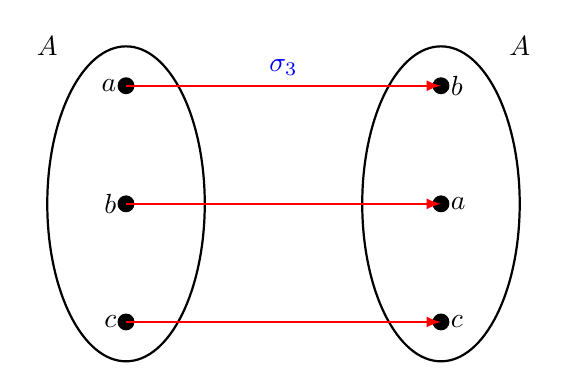
\begin{tikzpicture}[scale=1]
		% Coordenadas de puntos
		\coordinate (A0) at (0,1.5);
		\coordinate (A1) at (0,0);
		\coordinate (A2) at (0,-1.5);
		
		\coordinate (B0) at (4,1.5);
		\coordinate (B1) at (4,0);
		\coordinate (B2) at (4,-1.5);
		
		% Elipses
		\node at (-1, 2) {$A$};
		\node at (5, 2) {$A$};
		\draw[thick] (0,0) ellipse (1 and 2);
		\draw[thick] (4,0) ellipse (1 and 2);
		
		% Puntos
		\draw[fill] (A0) circle (1mm) node[left] {$a$};
		\draw[fill] (A1) circle (1mm) node[left] {$b$};
		\draw[fill] (A2) circle (1mm) node[left] {$c$};
		
		\draw[fill] (B0) circle (1mm) node[right] {$b$};
		\draw[fill] (B1) circle (1mm) node[right] {$a$};
		\draw[fill] (B2) circle (1mm) node[right] {$c$};
		
		% flechas
		\draw[red, thick, -latex] (A0) -- (B0) node[above, blue, midway]{$\sigma_3$};
		\draw[red, thick, -latex] (A1) -- (B1);
		\draw[red, thick, -latex] (A2) -- (B2);
	\end{tikzpicture}
	\caption{}
	\label{fig:permut}
\end{figure}

Si colocamos los elementos de $A$ en un triángulo equilátero, trazando bisectrices en cada ángulo, como se muestra en la fig. \ref{fig:gtriang}, cada elemento de $S_3$ puede entenderse como:
\begin{figure}[h]
	\centering
	\includestandalone[scale=2]{resources/ltx/grupoS3}
	\caption{}
	\label{fig:gtriang}
\end{figure}

\begin{itemize}
	\item Identidad: $i_A = \varepsilon$
	\item Reflexiones $(\sigma)$: respecto a cada bisectriz.
	\begin{itemize}
		\item Respecto de la bisectriz que pasa por $a$: $\sigma_1$ ($a$ es un \textbf{punto fijo})
		\item Respecto de $b$: $\sigma_2$ ($b$ es un punto fijo)
		\item Respecto de $c$: $\sigma_3$ ($c$ es un punto fijo)
	\end{itemize}
	\item Rotaciones $(\phi)$: los elementos \textit{giran}\footnote{El giro es de $60 \unit{\degree}$ (en general $360/n$), en sentido antihorario de acuerdo a cómo fueron colocados $a, b, c$ en la fig. \ref{fig:gtriang}} y se reubican en nuevos vértices.
	\begin{itemize}
		\item $\phi_1$: $a \mapsto b, b \mapsto c, c \mapsto a $, es decir:  $(a, b, c) \mapsto (b, c, a)$
		\item $\phi_2$: $a \mapsto c, c \mapsto b, b \mapsto a $, es decir: $(a, c, b) \mapsto (c, b, a)$
	\end{itemize}
\end{itemize}

\[ S_3 = \{ \varepsilon, \sigma_1, \sigma_2, \sigma_3, \phi_1, \phi_2\} \]

El conjunto $S_3$ se conoce como \textbf{simetrías del triángulo}, similarmente $S_4$ contiene las \textbf{simetrías del cuadrado}. En general las simetrías son transformaciones de reflexiones y rotaciones que mantienen las formas. Estas simetrías forman un grupo llamado \textbf{grupo de simetrías} $S_n$. Cuando la forma es un polígono regular el grupo de simetrías es llamado \textbf{grupo diédrico} $D_n$.

Utilizando números $A = \{1,2,3\}$ en sustitución de $\{a, b, c\}$ se tiene la tabla \ref{tab:S3}.
\begin{table}[h]
	\centering
	\begin{tabular}{|c|c|c|c|c|c|c|} \hline
		$A$ & $e$& $r$ & $r^2$ & $f$ & $rf$ & $r^2f$ \\ \hline
		1 & 1 & 3 & 2 & 1 & 2 & 3 \\ \hline
		2 & 2 & 1 & 3 & 3 & 1 & 2\\ \hline
		3 & 3 & 2 & 1 & 2 & 3 & 1\\ \hline
	\end{tabular}
	\caption{}
	\label{tab:S3}
\end{table}

En donde hemos llamado $r$ a una rotación y $f$ a una reflexión:
\[ \begin{array}{ccc}
	\varepsilon = e; & r = \phi_1; & r^2 = \phi_2;\\
	 f = \sigma_1; & rf = \sigma_3; & r^2f = \sigma_2
\end{array} \]

Los grupos de simetrías para diferentes triángulos son:

\begin{itemize}
	\item Equilátero: $\{ e, r, r^2, f, rf, r^2f \}$;
	\item Isósceles: $\{ e, f \}$;
	\item Escaleno: $\{ e \}$
\end{itemize}

\textbf{Tarea:}
Escribe el grupo de simetrías del cuadrado y del rectángulo.

\textbf{Composición de funciones en $S_3$}

Se muestra en la fig. \ref{fig:compos} un ejemplo de composición de funciones y en la tabla \ref{fig:compos} la composición de todos los pares de funciones, la operación es:

\[ \sigma_3 \circ \sigma_1 = \begin{pmatrix}
	1 & 2 & 3\\
	2 & 1 & 3
\end{pmatrix} \circ \begin{pmatrix}
	1 & 2 & 3\\
	1 & 3 & 2
\end{pmatrix} = \begin{pmatrix}
	1 & 2 & 3\\
	3 & 1 & 2
\end{pmatrix} = \phi_2\]

\begin{figure}[H]
	\centering
	\begin{tikzpicture}[scale=1]
		% Coordenadas de puntos
		\coordinate (A0) at (0,1.5);
		\coordinate (A1) at (0,0);
		\coordinate (A2) at (0,-1.5);
		
		\coordinate (B0) at (4,1.5);
		\coordinate (B1) at (4,0);
		\coordinate (B2) at (4,-1.5);
		
		\coordinate (C0) at (8,1.5);
		\coordinate (C1) at (8,0);
		\coordinate (C2) at (8,-1.5);
		
		% Elipses
		\draw[thick] (0,0) ellipse (1 and 2);
		\draw[thick] (4,0) ellipse (1 and 2);
		\draw[thick] (8,0) ellipse (1 and 2);
		
		% Puntos
		\draw[fill] (A0) circle (1mm) node[left] {$1$};
		\draw[fill] (A1) circle (1mm) node[left] {$2$};
		\draw[fill] (A2) circle (1mm) node[left] {$3$};
		
		\draw[fill] (B0) circle (1mm) node[right] {$2$};
		\draw[fill] (B1) circle (1mm) node[right] {$1$};
		\draw[fill] (B2) circle (1mm) node[right] {$3$};
		
		\draw[fill] (C0) circle (1mm) node[right] {$3$};
		\draw[fill] (C1) circle (1mm) node[right] {$1$};
		\draw[fill] (C2) circle (1mm) node[right] {$2$};
		
		% flechas
		\draw[red, thick, -latex] ($(A0)+(.4,0)$) -- ($(B0)+(-.4,0)$) node[above, blue, midway]{$\sigma_1$};
		\draw[red, thick, -latex] ($(A1)+(.4,0)$) -- ($(B1)+(-.4,0)$);
		\draw[red, thick, -latex] ($(A2)+(.4,0)$) -- ($(B2)+(-.4,0)$);
		
		\draw[red, thick, -latex] ($(B0)+(.5,0)$) -- ($(C0)+(-.4,0)$) node[above, blue, midway]{$\sigma_3$};
		\draw[red, thick, -latex] ($(B1)+(.5,0)$) -- ($(C1)+(-.4,0)$);
		\draw[red, thick, -latex] ($(B2)+(.5,0)$) -- ($(C2)+(-.4,0)$);
		
		\draw[blue, very thick, -latex] ($(A2)+(.4,-.3)$) to[bend right=20] ($(C2)+(-.4, -.3)$) node[below, xshift=-60, yshift=-20] {$\phi_2=\sigma_3 \circ \sigma_1$};
	\end{tikzpicture}
	\caption{}
	\label{fig:compos}
\end{figure}

\begin{table}[H]
	\centering
	\begin{tabular}{c|cccccc}
		$\circ$ & $\varepsilon$ & $\sigma_1$ & $\sigma_2$ & $\sigma_3$ & $\phi_1$ & $\phi_2$ \\ \hline
		$\varepsilon$ & $\varepsilon$ & $\sigma_1$ & $\sigma_2$ & $\sigma_3$ & $\phi_1$ & $\phi_2$ \\
		$\sigma_1$ & $\sigma_1$ & $\varepsilon$ & $\phi_1$ & $\phi_2$ & $\sigma_2$ & $\sigma_3$ \\
		$\sigma_2$ & $\sigma_2$ & $\phi_2$ & $\varepsilon$ & $\phi_1$ & $\sigma_3$ & $\sigma_1$\\
		$\sigma_3$ & $\sigma_3$ & $\phi_1$ & $\phi_2$ & $\varepsilon$ & $\sigma_1$ & $\sigma_2$\\
		$\phi_1$ & $\phi_1$ & $\sigma_3$ & $\sigma_1$ & $\sigma_2$ & $\phi_2$ & $\varepsilon$\\
		$\phi_2$ & $\phi_2$ & $\sigma_2$ & $\sigma_3$ & $\sigma_1$ & $\varepsilon$ & $\phi_1$\\
	\end{tabular}
	\caption{Grupo $(S_3, \circ)$.}
	\label{tab:compos}
\end{table}

\begin{itemize}
	\item[G1:] Asociatividad \cmark
	\item[G2:] Elemento neutro: $\varepsilon$ \cmark
	\item[G3:] Inversos: \cmark
	\begin{itemize}
		\item Todos son sus propios inversos a excepción de $\phi_1$ y $\phi_2$ que son inversos entre si.
	\end{itemize}
	\item[G4:] Conmutatividad: \xmark
\end{itemize}

\subsection{Subgrupos} \label{sec:subgrupo}
\vspace{3mm}	
	\begin{fmd-definition}[Subgrupo]
		El subconjunto no vacío $H$ de $G$, es un subgrupo de $(G, *)$ si y solo si $(H, *)$ es un grupo.
	\end{fmd-definition}
	Notar que como el neutro es único y $H \subseteq G \implies e_G = e_H$
	
	\textbf{Subgrupos}:
	\begin{enumerate}
		\item $(\mathbb{Z}, +) \le (\mathbb{Q}, +) \le (\mathbb{R}, +) \le (\mathbb{C}, +)$
		\item $\left( \{1, -1 \}, \bdot \right) \le \left( \mathbb{Q} \setminus \{0\}, \bdot \right) \le \left( \mathbb{R} \setminus \{0\}, \bdot \right) \le \left( \mathbb{C} \setminus \{0\}, \bdot \right)$
	\end{enumerate}
	
	\begin{fmd-theorem}[Condición suficiente para existencia de subgrupo] \label{teo:subgrupo}
		Dado el grupo $(G, *)$, si $H \subseteq G$, con $H \ne \emptyset$, que verifica:
		\[ a \in H \land b \in H \implies a * b' \in H\]
		entonces $(H, *)$ es un subgrupo de $(G, *)$.
	\end{fmd-theorem}

	\begin{fmd-proof}
		\begin{itemize}
			\item Asociatividad: se verifica por ser $H \subset G$.
			\item El neutro pertenece a $H$. En efecto: $H \ne \emptyset \implies \exists a \in H$
			\vspace{-3mm}
			\[a \in H \land a \in H \implies a*a'\in H \implies e \in H\]
			\item Todo elemento de $H$ admite inverso en $H$.
			\vspace{-3mm}
			\[ e \in H \land a \in H \implies e * a' \in H \implies a'\in H \]
			\item $H$ es cerrado para $*$
			\vspace{-3mm}
			\[ a \in H \land b \in H \implies a \in H \land b' \in H \implies a*(b')' \in H \implies \]
			\[ a*b \in H\]
		\end{itemize}
	\end{fmd-proof}
	Es fácil verificar que la condición también es necesaria.
	
Observemos que los enteros pares forman subgrupo de $(\Z, +)$ pero los impares no ?`por qué?

\begin{definition}[Subgrupo trivial]
	Sea $(G, *)$ un grupo no vacío, consideremos el conjunto $H = \{ e \}$, claramente $H \subset G$, se cumple que $(H, *)$ es un subgrupo de $(G, *)$, pues:
	\[ e \in H \land e \in H \implies e * e' = e \in H \]
	
	Al subgrupo $(H, *)$ definido de esta manera se le llama \textit{subgrupo trivial}.
\end{definition}

\begin{fmd-definition}[Subgrupo cíclico]
	Sea $(G, *)$ un grupo y $a \in G$, consideremos el conjunto $H = \{ a^n: n \in \mathbb{Z}\}$, $(H, *)$ es un subgrupo de $(G, *)$.
	
	\begin{proof}
		Sean $g, h \in H$ entonces $ \exists m, n \in \mathbb{Z} / g = a^m \land h = a^n$, en consecuencia $g*h^{-1} = a^m * a^{-n} = a^{m-n} \in H $
		así tenemos que $(H, *)$ es un subgrupo de $(G,*)$
	\end{proof}
	Notemos que si $a=1_G$ entonces $H=\{a^n:n \in \mathbb{Z}\} = \{1_G\}$, pero si $a\neq 1_G$ en $H$ tenemos al menos dos elementos:
	\[ a = a^1 \mbox{ y } 1_G = a^0 \]
	Al subgrupo $(H, *)$ se le llama \textit{subgrupo cíclico} generado por $a$ y se denota por
	\[ H = \langle a \rangle \]
\end{fmd-definition}
	
	Sea $G$ un grupo y $a \in G$:
	\begin{itemize}
		\item \textbf{Notación multiplicativa}:
		\[ a^1 = a, \; a^0 = 1, \; a^n = \underbrace{a \cdots a}_{n \, veces}, \forall n \ge 2; \quad a^{-n} = (a^{-1})^n = \underbrace{a^{-1} \cdots a^{-1}}_{n \, veces}\] \vspace{-5mm}
		
		\item \textbf{Notación aditiva}:
		\[ 1a = a, \; 0a = 0, \; na = \underbrace{a + \cdots + a}_{n \, veces}, \forall n \ge 2; \quad -na = \underbrace{-a - \cdots -a}_{n \; veces}\]
	\end{itemize}
	
	\begin{fmd-example}
		El grupo $(\mathbb{Z}, +)$ es cíclico, pues cualquier elemento $p \in \mathbb{Z}$ es de la forma: $p = 1^p = \underbrace{1+1+\cdots+1}_{p \, veces} = 1 \cdot p$
	\end{fmd-example}
	
	$\mathbb{Q}, \mathbb{R}$ y $\mathbb{C}$ no son cíclicos. El grupo de números pares $\langle 2 \rangle$ es cíclico. El menor grupo cíclico es el trivial.
	
	Utilizando la notación multiplicativa los subgrupos cíclicos con generador $x$ deben ser de la forma:
	\[ \langle x \rangle = \{ \dots, x^{-3}, x^{-2}, x^{-1}, 1, x, x^2, x^3,  \dots \} \]
	
	En la notación aditiva tenemos:
	\[ \langle y \rangle = \{ \dots, -3y, -2y, -y, 0, y, 2y, 3y,  \dots \} \]


	\begin{fmd-definition}[Orden de un elemento]
		Sean $(G, *)$ un grupo y $a \in G$. Consideremos al conjunto $\{ n \in \mathbb{Z}^{+}: a^n = 1_G \}$. Se define el \textit{orden} de $a$ como:
		\[ o(a) = |a| = \min \{ n \in \mathbb{Z}^{+}: a^n = 1_G\} \in \mathbb{Z}^{+} \]
		en este caso diremos que $a$ es de orden finito.
		
		Si $\{ n \in \mathbb{Z}^{+}: a^n = 1_G\} = \emptyset$ definimos el orden de $a$ como $o(a) = \infty$.
	\end{fmd-definition}
	\begin{itemize}
		\item Notar que $o(1_G) = 1$ y es único, i.e., $\exists! \, a \in G$ con $o(a) = 1$ ($a = 1_G$).
		\item El orden del generador coincide con el del subgrupo cíclico que genera:
		\[ o(a) = |\langle a \rangle| \]
	\end{itemize}
	
	\begin{fmd-example}
		Sea $G = \{ 1, i, -1, -i \}$ siendo $i = \sqrt{-1}$ la unidad imaginaria. Su tabla de Cayley para la operación de multiplicación es:
		\[ \begin{array}{r|rrrr}
			\times & 1 & i & -1 & -i\\ \hline
			1 & 1 & i & -1 & -i\\
			i & i & -1 & -i & 1\\
			-1 & -1 & -i & 1 & i\\
			-i & -i & 1 & i & -1 
		\end{array} \]
		Notar que el grupo es abeliano y cíclico, generado por $i$, es decir $G = \langle i \rangle$. El elemento neutro es el 1.
		
		El orden del elemento $-1$ es 2, porque $(-1)^2 = 1$, el orden del elemento generador $i$ es 4, porque $i^4 = 1$, que es igual al orden $|G|$ del subgrupo generado.
	\end{fmd-example}
	
	\begin{fmd-example}
		Considerando el grupo de simetrías del triángulo equilátero $D_3 = \{ e, r, r^2, f, rf, r^2f \}$, en donde $r$ es una rotación y $f$ una reflexión.
		
		Como $r^3 = e$ el orden de $r$ es $|r| = 3$, análogamente, como $f^2 = e$ el orden de $f$ es $|f| = 2$.
	\end{fmd-example}
	
	\textbf{Tarea}: Probar que:
	\begin{enumerate}
		\item Si un grupo es cíclico, entonces es abeliano.
		\item Cualquier subgrupo de un  grupo cíclico, también es cíclico.
		\item Cualquier grupo $(G, \bdot)$ de orden 1, 2, 3 o 4 es abeliano
	\end{enumerate}

	Sean $(G, *)$ un grupo y $\{G_i\}_{i \in I}$ una familia de subgrupos de $(G, *)$
	\begin{fmd-theorem}
		La intersección de toda familia no vacía de subgrupos de $(G, *)$ es un subgrupo.
	\end{fmd-theorem}
	
	\begin{fmd-proof}
		\begin{itemize}
			\item[H)] $(G, *)$ es grupo. $\{G_i\}$ es tal que $(G, *)$ es un subgrupo de $G, \forall i \in I$.
			\item[T)] $\left( \bigcap_{i \in I} G_i, * \right)$ es subgrupo de $(G, *)$
		\end{itemize}
		\begin{enumerate}[label=\roman*)]
			\item $\forall i: e \in G_i$, pues $(G_i, *)$ es un grupo: $e \in \bigcap_{i \in I} G_i \implies \bigcap_{i \in I} G_i \ne \emptyset$
			\item $\bigcap_{i \in I} G_i \subset G$ por definición de inclusión
			\item Sean $a, b \in \bigcap_{i \in I}G_i \implies a \in G_i \land b \in G_i, \forall i \implies$
			
			$a * b'\in G_i, \forall i \implies a * b' \in \bigcap_{i \in I}G_i$
		\end{enumerate}
	\end{fmd-proof}
	Esta propiedad no se verifica en el caso de la unión.

	\begin{fmd-definition}[Núcleo de homomorfismo]
		Núcleo o \textit{kernel} del homomorfismo $f: G \rightarrow G'$ es la totalidad de los elementos de $G$, cuyas imágenes por $f$ se identifican con el neutro de $G'$.
		\[ N(f) = \ker f = \{ x \in G / f(x) = e' \} \]
	\end{fmd-definition}
	Es claro que el núcleo de $f$ es la preimagen de $e'$.
	
\begin{figure}[H]
	\centering
	\includestandalone[scale=1.1]{resources/ltx/kernel}
	\caption{}
	\label{fig:kernel}
\end{figure}

	\begin{proposition}
		El núcleo de todo homomorfismo de grupos es un subgrupo del primero.
	\end{proposition}
	\begin{proof}
		En efecto:
		\begin{itemize}
			\item $\forall a, b \in \ker f \implies f(ab) = f(a)f(b) = e_{G'} e_{G'} = e_{G'} \implies ab \in \ker f$.
			\item $a \in \ker f \implies f(a^{-1}) = \left[ f(a) \right]^{-1}=e_{G'}^{-1} = e_{G'} \implies a^{-1} \in \ker f$
		\end{itemize}
	\end{proof}
	
	\begin{proposition}
		El homomorfismo $f: G \rightarrow G'$ es inyectivo, es decir, un monomorfismo si y solo si el núcleo es unitario: $\ker(f) = \{ e\}$.
	\end{proposition}
	\begin{proof}:
		\begin{itemize}
			\item Si $f$ es inyectivo, entonces $\forall a \in G \land a \ne e_G$ debemos tener $f(a) \ne f(e_G) = e_G$, es decir, $\ker f = \{e_G\}$;
			\item Recíprocamente, si $\ker f = \{ e_G\}$, entones: $f(a) = f(b) \implies f(a) \left[f(b)\right]^{-1} = e_H \implies f(ab^{-1}) = e_H \implies ab^{-1}=e_G \implies a=b$
		\end{itemize}
	\end{proof}


	\begin{fmd-definition}[Imagen de un homomorfismo]
		Es la totalidad de las imágenes de los elementos del primer grupo.
	\end{fmd-definition}
	
	\begin{proposition}
		La imagen de todo homomorfismo de grupos es un subgrupo del segundo: $Im(f) \subseteq G'$.
	\end{proposition}


	\begin{definition}[Subgrupo distinguido]
		El subgrupo $(H, *)$ de $(G, *)$ es \textbf{distinguido} si y sólo si existe un grupo $(G', *')$ y un homomorfismo $f: G \rightarrow G'$, cuyo núcleo es $H$.
		
		En símbolos:
		
		$H \subset G$ es distinguido $\iff \exists G'$ grupo, y $f:G \rightarrow G'$ homomorfismo $/ N(f) = H$
	\end{definition}
	
	Subgrupos distinguidos de todo grupo $(G, *)$ son el mismo $G$ y $\{e\}$ \cite{rojoAlgebra8vaEd} p249.

\subsection{Subgrupo normal} \label{sec:subgrupo_normal}

	\subsubsection{Relación de equivalencia y clases}
	
	Sea $(H, *)$ un subgrupo de $(G, *)$. Definimos en $G$ la relación $\sim$ mediante: $a \sim b \iff a' * b \in H$, es decir, dos elementos está relacionados si y sólo si la composición del inverso del primero con el segundo pertenece a $H$.
	
	La relación es de equivalencia pues verifica la reflexividad $a \sim a$, simetría $a\sim b \implies b \sim a$ y transitividad $a\sim b \land b \sim c \implies a \sim c$, en efecto
	
	\begin{fmd-proof} Propiedades de equivalencia:
		\begin{enumerate}[label=\roman*)]
			\item Reflexividad: $a \equiv_{H} a \iff aa^{-1} = e \in H$;
			\item Simetría: Si $a \equiv_{H} b \implies ab^{-1} \in H$ luego $(ab^{-1})^{-1} \in H$, así $ba^{-1} \in H$. De modo que $b \equiv_{H} a$
			\item Transitividad: Sean $a \equiv_{H} b$ y $b \equiv_{H} c$ luego $ab^{-1}, bc^{-1} \in H$ multiplicando ambos elementos $\left(ab^{-1}\right) \left(bc^{-1}\right) = aec^{-1} = ac^{-1} \in H$. Se tiene que $a \equiv_{H} c$.
		\end{enumerate}
		Concluimos que $a \equiv_{H} b$ es una relación de equivalencia.
	\end{fmd-proof}
	
	\textbf{Algunas definiciones} $\forall a \in G \land H \subseteq G$:
	\begin{itemize}
		\item \textbf{Conjugado}: Para $a,b, g \in G$, se dice que $b$ es el \textbf{conjugado} de $a$ por $g$ si existe este elemento $g$ tal que $b = g^{-1}ag$.
		\item \textbf{Clase\footnote{Algunos autores utilizan los términos: \textit{coclase} o \textit{cogrupo} en vez de \textit{clase}.} lateral izquierda de H}: es el subgrupo $aH \coloneqq \{ah; h \in H\} $
		\item \textbf{Clase lateral derecha de H}: es el subgrupo $Ha \coloneqq \{ha; h \in H\} $
		\item \textbf{Grupo conjugado\footnote{Otros llaman \textit{coclases} a las clases laterales y \textit{clases} a los grupos conjugados.} de H}: es el subgrupo $a^{-1}Ha \coloneqq \{a^{-1}ha; h \in H\} $
		\item \textbf{Centro de G}: $Z(G) \coloneqq \{z\in G / zx = xz \forall x \in G\}$. Subgrupo que contiene todos los elementos que conmutan con cualquier elemento de $G$.
	\end{itemize}
	
	\begin{fmd-definition}[Subgrupo normal o invariante] \label{def:normal}
		El subgrupo $(H, *)$ de $(G, *)$ es normal o invariante, si y solo si se verifica: $ x \in G \land y \in H \implies x * y * x^{-1} \in H $
	\end{fmd-definition}
	
	En otras palabras, en un grupo normal, el conjugado de un elemento de $H$ pertenece a $H$.
	
	\textbf{Notas}:
	\begin{enumerate}
		\item Notación: $H \triangleleft G$ se lee \textit{$H$ es un subgrupo normal} (o invariante) de $G$;
		\item En toda $G$ siempre existen por lo menos dos subgrupos normales:
		\begin{itemize}
			\item El subgrupo trivial: $\{e\}$;
			\item El grupo entero: $G$
		\end{itemize}
		\item Un subgrupo es distinguido si y sólo si es invariante.
	\end{enumerate}
	
	\begin{proposition}[Subgrupos de grupos abelianos] \label{prop:subgrupo}
		Todo subgrupo de un grupo abeliano es normal, es decir: $\forall x, y: x\in G \land y \in H \implies xyx^{-1} = xx^{-1}y = ey = y \in H$;
	\end{proposition}
	
	\begin{definition}[Grupo simple]
		Un \textbf{grupo simple} es un grupo no trivial con exactamente dos subgrupos normales, el subgrupo trivial y él mismo.
	\end{definition}
	
	\begin{proposition}
		Si $f: G \rightarrow H$ es un homomorfismo, entonces $\ker f \subseteq G$ es un subgrupo normal. \[ \ker f \trianglelefteq G \]
	\end{proposition}
	
	\begin{proof}
		En efecto: $\forall a \in G \land b \in \ker f$
		\[f(a^{-1}ba) = f(a^{-1}) f(b) f(a) = f^{-1}(a) e_H f(a) = f^{-1}(a)f(a) = e_H\]
		así:
		\[a^{-1} (\ker f) a \in \ker f\]
	\end{proof}
	
	La definición \ref{def:normal} es equivalente a decir que si  $H$ es un subgrupo normal de $G$, entonces las clases laterales izquierda y derecha de $H$ son iguales, es decir:
	\begin{equation} \label{eq:normal}
		H \triangleleft G \implies gH = Hg
	\end{equation}
	La expresión $Hg$ no es otra cosa que operar $h * g = hg \, \forall \, h \in H$ y $g \in G$.
	
	\begin{fmd-example}
		Recordemos el grupo $(S_3, \circ)$ con la tabla \ref{tab:compos}, que reescribimos aquí:
		\begin{table}[H]
			\centering
			\begin{tabular}{c|cccccc}
				$\circ$ & $\varepsilon$ & $\sigma_1$ & $\sigma_2$ & $\sigma_3$ & $\phi_1$ & $\phi_2$ \\ \hline
				$\varepsilon$ & $\varepsilon$ & $\sigma_1$ & $\sigma_2$ & $\sigma_3$ & $\phi_1$ & $\phi_2$ \\
				$\sigma_1$ & $\sigma_1$ & $\varepsilon$ & $\phi_1$ & $\phi_2$ & $\sigma_2$ & $\sigma_3$ \\
				$\sigma_2$ & $\sigma_2$ & $\phi_2$ & $\varepsilon$ & $\phi_1$ & $\sigma_3$ & $\sigma_1$\\
				$\sigma_3$ & $\sigma_3$ & $\phi_1$ & $\phi_2$ & $\varepsilon$ & $\sigma_1$ & $\sigma_2$\\
				$\phi_1$ & $\phi_1$ & $\sigma_3$ & $\sigma_1$ & $\sigma_2$ & $\phi_2$ & $\varepsilon$\\
				$\phi_2$ & $\phi_2$ & $\sigma_2$ & $\sigma_3$ & $\sigma_1$ & $\varepsilon$ & $\phi_1$\\
			\end{tabular}
		\end{table}
		
		El conjunto $H = \{\varepsilon, \sigma_1\}$ es un subgrupo de $S_3$, sus clases a derecha e izquierda son:
		
		\begin{table}[H]
			\centering
			\begin{tabular}{c|c}
				Clases a derecha & Clases a izquierda\\ \hline
				$H = \{\varepsilon, \sigma_1\}$ & $H = \{ \varepsilon, \sigma_1 \}$\\
				$H\phi_1 = \{ \phi_1, \sigma_2 \}$ & $\phi_1H = \{ \phi_1, \sigma_3 \}$\\
				$H\phi_2 = \{ \phi_2, \sigma_3 \}$ & $\phi_2H = \{ \phi_2, \sigma_2 \}$
			\end{tabular}
		\end{table}
		Se observa que las clases a derecha e izquierda no son iguales, por tanto, $H$ no es un subgrupo normal de $S_3$.
	\end{fmd-example}
	
	\begin{fmd-definition}[Producto de clases laterales]
		Sea $H \triangleleft G$ y sean $Ha$ y $Hb$ clases laterales de $H$ definimos el producto de clases laterales derechas como $ (Ha) (Hb) = Hab $.
	\end{fmd-definition}
	Veamos si este producto está bien definido.
	\begin{fmd-proof}
		Sean $a_1, a_2 \in Ha$ y $b_1, b_2 \in Hb$ se debe probar que $a_1b_1 \in Hab$ y $a_2b_2 \in Hab$ o, lo que es lo mismo, $a_1b_1 \equiv_{H} a_2b_2$.
		
		Se tiene que, si
		\[ a_1 \in Ha \, \exists \, h_1 \in H \, | \, a_1 = h_1a_2, \quad b_1 \in Hb \, \exists \, h_2 \in H \, | \, b_1 = h_2b_2 \]
		luego:
		\[ a_1b_1 = (h_1a_2)(h_2b_2) = h_1 (a_2 h_2) b_2 \]
		pero por ser $H$ un subgrupo normal $Hg = gH \, \forall g \in G$, así
		\[ a_1b_1 = h_1(a_2h_2)b_2 = h_1(h_3a_2)b_2 = (h_1h_3)a_2b_2 \implies (a_1b_1)(a_2b_2)^{-1} = h_1h_3 \in H \] 
	\end{fmd-proof}

\subsection{Grupo cociente}
\vspace{1em}
\begin{fmd-theorem}[Grupo cociente] \label{teo:cociente}
	Si $H \triangleleft G$ y sea el conjunto $G/H = \{ \bar{g} / g \in G \} = \{ Hg / g \in G \}$, entonces $G/H$ es un grupo bajo la operación $(Ha)(Hb) = Hab, \forall a, b \in G$.
\end{fmd-theorem}

\begin{fmd-definition}[Grupo cociente]
	El grupo $(G/H, *)$ a que se refiere el teorema \ref{teo:cociente} se llama grupo cociente de $G$ por la relación de equivalencia compatible con $*$.
\end{fmd-definition}

\textbf{Notas}
\begin{itemize}
	\item $G/\{e\} = G$;
	\item $G / G = \{ e \}$
\end{itemize}

\begin{fmd-example} \label{ex:cociente}
	$(\Z, +)$ es un grupo abeliano. Sea $H$ el conjunto de los múltiplos de 5, esto es, $H = \{ \dots, -10, -5, 0, 5, 10, \dots \}$. Las clases laterales izquierda de $H$ en $\Z$ son:
	\[ \begin{array}{l}
		\bar{0} = 0 + H = \{ \dots, -10, -5, 0, 5, 10, \dots \}\\
		\bar{1} = 1 + H = \{ \dots, -9, -4, 1, 6, 11, \dots \}\\
		\bar{2} = 2 + H = \{ \dots, -8, -3, 2, 7, 12, \dots \}\\
		\bar{3} = 3 + H = \{ \dots, -7, -2, 3, 8, 13, \dots \}\\
		\bar{4} = 4 + H = \{ \dots, -6, -1, 4, 9, 14, \dots \}
	\end{array} \]
	
	Notar que las clases laterales derecha $\bar{x} = H + x$ serán iguales a las izquierdas, por tanto, $(H, +)$ es un subgrupo normal, $H \triangleleft \Z$.
	
	Para cualquier otro entero $n \in \Z$, $\bar{n} = n + H$ coincide con una de las clases anteriores. Luego, el grupo cociente $\Z / H = \{ \bar{0}, \bar{1}, \bar{2}, \bar{3}, \bar{4} \}$ forma un grupo para la adición según el teorema \ref{teo:cociente}. La siguiente es la tabla de adición:
	\begin{table}[H]
		\centering
		\[
		\begin{array}{c|ccccc}
			+ & \bar{0} & \bar{1} & \bar{2} & \bar{3} & \bar{4}\\ \hline
			\bar{0} & \bar{0} & \bar{1} & \bar{2} & \bar{3} & \bar{4}\\
			\bar{1} & \bar{1} & \bar{2} & \bar{3} & \bar{4} & \bar{0}\\
			\bar{2} & \bar{2} & \bar{3} & \bar{4} & \bar{0} & \bar{1}\\
			\bar{3} & \bar{3} & \bar{4} & \bar{0} & \bar{1} & \bar{2}\\
			\bar{4} & \bar{4} & \bar{0} & \bar{1} & \bar{2} & \bar{3}\\
		\end{array}
		\]
	\end{table}
\end{fmd-example}

\subsubsection{Grupos finitos}

Se G un grupo. Por definición $G$ es finito si y sólo si $|G| = n$. Orden de un grupo finito es el número cardinal del mismo.

\begin{fmd-definition}[Índice de un subgrupo]
	Sea $H$ un subgrupo del grupo finito $G$. El grupo cociente $G/H$, de las clases a izquierda de $H$, es finito y su cardinal se llama \textbf{índice del subgrupo} $H$ en $G$.
\end{fmd-definition}

El índice de $H$ en el ejemplo \ref{ex:cociente} es igual a $|\Z/H| = 5$.

\begin{fmd-theorem} \label{teo:finito}
Si $H$ es un subgrupo de orden $k$ del grupo finito $G$, entonces toda clase izquierda de $H$ tiene $k$ elementos.

\begin{itemize}
	\item[H)] $(G, *)$ es grupo finito; $|H| = k$.
	\item[T)] $|gH| = k \; \forall g \in G$.
\end{itemize}
\end{fmd-theorem}
\begin{fmd-proof}
	Debemos probar que $H$ y $gH$ son coordinables, y para ello difinimos:
	\[ f: H \rightarrow gH \mbox{ mediante } f(a) = g * a \]
	\begin{enumerate}[label=\roman*)]
		\item $f$ es la restricción de la \textit{translación a izquierda} $f_g: G \rightarrow G$ al subconjunto $H$ y en consecuencia es inyectiva.
		\item $f$ es sobreyectiva, pues para todo $y \in gH$ existe $x = g'*y$ tal que:
		\[ f(x) = f(g' * y) = g * g' * x = x \]
	\end{enumerate}
	En consecuencia, $f$ es biyectiva y $|gH| = |H| = k$
\end{fmd-proof}

\begin{fmd-theorem}[Lagrange] \label{teo:Lagrange}
	El orden de todo subgrupo de un grupo finito es divisor del orden del grupo.
\end{fmd-theorem}

\begin{fmd-proof} En efecto:
	
	Si $H$ es un subgrupo  de $G$ y $o(H) = k$ por el teorema \ref{teo:finito} el cardinal de toda coclase a izquierda de $H$ es $k$, y como estas son disjuntas, resulta:
	\[ o(G) = mk = m o(H) \]
	es decir:
	\[ o(H) \mid o(G) \]
\end{fmd-proof}



\subsection{Aritmética modular} \label{sec:aritmod}

La aritmética modular es un sistema aritmético para clases de equivalencia de números enteros llamadas \textbf{clases de congruencia}. Es uno de los aportes más significativos de Gauss a la Teoría de Números, en su famoso Disquisitiones Arithmeticae (Investigaciones sobre aritmética) de 1801.

Consideremos el ``reloj'' de la fig \ref{fig:relojMod3}. Se conoce como \textit{enteros módulo} 4 al conjunto $\Z_4 = \{ 0, 1, 2, 3 \}$.
\begin{figure}[h]
	\centering
	\includestandalone[scale=1.5]{resources/ltx/relojMod3}
	\caption{Enteros módulo 4}
	\label{fig:relojMod3}
\end{figure}

Veamos las operaciones de suma y multiplicación en $\Z_4$.

\subsubsection{Suma}

Para la operación suma se tienen los valores de la tabla \ref{tab:mod4}.
\begin{table}[h]
	\centering
	\begin{tabular}{c|cccc}
		$+$ & 0 & 1 & 2 & 3\\
		\hline
		0 & 0 & 1 & 2 & 3\\
		1 & 1 & 2 & 3 & 0\\
		2 & 2 & 3 & 0 & 1\\
		3 & 3 & 0 & 1 & 2\\
	\end{tabular}
	\caption{Enteros módulo 4 con la operación suma. Es un grupo abeliano.}
	\label{tab:mod4}
\end{table}

La operación es cerrada ya que:
\[ +: \Z_4 \times \Z_4 \rightarrow \Z_4  \]
\[ \mbox{Ejm: observando la tabla \ref{tab:mod4}} (1,3) \rightarrow 0 \]

\begin{itemize}
	\item[G1:] Es asociativa \cmark
	\item[G2:] Elemento neutro: 0 \cmark
	\item[G3:] Inversos: \cmark  \begin{itemize}
		\item 0 es su propio inverso;
		\item 2 es su propio inverso;
		\item 1 y 3 son inversos.
	\end{itemize}
	\item[G4:] Es conmutativa \cmark
\end{itemize}

\begin{center}
	$(\Z_4, +)$ es un grupo abeliano y finito.
\end{center}

En general, para los enteros múdulo $n$ con la operación suma:
\begin{center}
	$(\Z_n, +)$ es un grupo abeliano finito.
\end{center}

\subsubsection{Producto}

\begin{itemize}
	\item $(\Z_4, \bdot)$
	
	Para la operación producto se tienen los valores de la tabla \ref{tab:mod4p}.
	\begin{table}[H]
		\centering
		\begin{tabular}{c|cccc}
			$\bdot$ & 0 & 1 & 2 & 3\\
			\hline
			0 & 0 & 0 & 0 & 0\\
			1 & 0 & 1 & 2 & 3\\
			2 & 0 & 2 & 0 & 2\\
			3 & 0 & 3 & 2 & 1\\
		\end{tabular}
		\caption{Conjunto de enteros módulo 4 con la operación producto.}
		\label{tab:mod4p}
	\end{table}
	
	\begin{itemize}
		\item[G1:] Es asociativa \cmark
		\item[G2:] Elemento neutro: 1 \cmark
		\item[G3:] Inversos: \xmark
	\end{itemize}
	
	\begin{center}
		$(\Z_4, \bdot)$ no es un grupo, es un semigrupo con neutro.
	\end{center}
	
	\item $(\Z^{*}_4, \bdot)$
	
	Si se excluye el cero, se tiene la tabla \ref{tab:mod4pa}.
	
	\begin{table}[H]
		\centering
		\begin{tabular}{c|cccc}
			$\bdot$ & 1 & 2 & 3\\
			\hline
			1 & 1 & 2 & 3\\
			2 & 2 & 1 & 3\\
			3 & 3 & 3 & 1
		\end{tabular}
		\caption{Enteros módulo 4, excluyendo el cero $(\Z^{*}_4, \cdot)$.}
		\label{tab:mod4pa}
	\end{table}
	
	\begin{itemize}
		\item[G1:] Es asociativa \cmark
		\item[G2:] Elemento neutro \xmark
	\end{itemize}
	
	\begin{center}
		$(\Z^{*}_4, \bdot)$ no es un grupo, es un semigrupo.
	\end{center}
	
	\item $(\Z^{*}_3, \bdot)$
	
	Si se excluye el cero, se tiene la tabla \ref{tab:mod3pa}.
	
	\begin{table}[H]
		\centering
		\begin{tabular}{c|cccc}
			$\bdot$ & 1 & 2\\
			\hline
			1 & 1 & 2 \\
			2 & 2 & 1\\
		\end{tabular}
		\caption{Enteros módulo 3, excluyendo el cero $(\Z^{*}_3, \bdot)$.}
		\label{tab:mod3pa}
	\end{table}
	
	\begin{itemize}
		\item[G1:] Es asociativa \cmark
		\item[G2:] Elemento neutro: 1 \cmark
		\item[G3:] Elemento inverso: \cmark
		\begin{itemize}
			\item 1 es su propio inverso;
			\item 2 es su propio inverso
		\end{itemize}
		\item[G4:] Es conmutativa: \cmark
	\end{itemize}
	
	\begin{center}
		$(\Z^{*}_3, \bdot)$ es un grupo abeliano.
	\end{center}
\end{itemize}

\begin{proposition} \label{prop:primo}
	$(\Z_p^{*}, \bdot)$ es un grupo multiplicativo abeliano si y sólo si $p$ es primo.
\end{proposition}

Observemos ahora la fig. \ref{fig:relojconrecta} imaginando el giro sin deslizar de la rueda, vemos que los números enteros tienen relación con $0, 1, 2$ o $3$ dependiendo de su posición, esta relación es de congruencia.

\begin{figure}[H]
	\centering
	\includestandalone[scale=.9]{resources/ltx/reloj-con-recta}
	\caption{}
	\label{fig:relojconrecta}
\end{figure}

Notemos que a cada $x \in \Z$ le corresponderá el elemento de $\Z_4$ que resulta de tomar el residuo de la división de $x$ entre 4. Los posibles residuos de la división de un entero entre 4 son 0, 1, 2, 3, en general:

Por lo tanto, podemos decir que todos los números de $\Z$ con el mismo residuo de la división entre 4 serán equivalentes (se puede verificar fácilmente que cumple con las propiedades de equivalencia), se dice que son congruentes módulo 4.

Por ejemplo:
\[ 4753 \equiv 1 \, (\mbox{mod } 4); \qquad 1234 \equiv 2 \, (\mbox{mod } 4) \]

\emph{Dos enteros $a, b \in \Z$ son congruentes módulo $n$ si al dividir entre $n$ dan el mismo residuo}.

\begin{fmd-proposition}
	La congruencia módulo $n$, con $n$ entero positivo fijo, es una relación de equivalencia.
\end{fmd-proposition}

\emph{Los enteros módulo $n$ pueden considerarse como el conjunto de clases que se forman con la relación de congruencia.}

Por la definición de división sabemos que el dividendo es igual al cociente por el divisor más el residuo, por lo tanto, para dos números $x, y$ congruentes módulo $n$ ($x, y$ tienen el mismo residuo), se tiene

\[ \begin{array}{c}
	x = c_1n + r \\
	y = c_2n + r \\ \hline
	x - y = (c_1 - c_2)n
\end{array} \]

en consecuencia, $x, y$ son congruentes módulo $n$ si y sólo si $n$ divide a $x - y$.
\[ x \equiv_{n} y \iff n \mid x - y \]

El conjunto de números con el mismo residuo $r$ son las \textbf{clases} de $r$, en el caso de $\Z_3$, estas son:
\[ \begin{split}
	\mbox{clase del 0}: \quad [0] = \bar{0} =& \{\dots, -6, -3, 0, 3, 6, \dots \}\\
	\mbox{clase del 1}: \quad [1] = \bar{1} =& \{\dots, -5, -2, 1, 4, 7, \dots \}\\
	\mbox{clase del 2}: \quad [2] = \bar{2} =& \{\dots, -4, -1, 2, 5, 8, \dots \}\\
\end{split} \]

Se observa que hablar de, por ejemplo, la clase $\bar{4}$ es lo mismo que hablar de la clase $\bar{1}$, ya que están el mismo conjunto. Además, llamamos a 1 \textbf{representante} de la clase $\bar{1}$, 2 representante de la clase $\bar{2}$, etc.

Llamemos $3\Z$ al conjunto formado por los múltiplos de 3, en general $n\Z$ al conjunto formado por los múltiplos de $n$.

$\bar{0}$ es el conjunto de todos los múltiplos de 3 $(3\Z)$, o lo que es lo mismo, el conjunto de todos los números que al dividir entre 3 dan resto nulo. $\bar{1}$ son todos los números enteros tales que al dividir entre 3 dan resto 1, análogamente para $\bar{2}$.

Se observa que $\Z/3\Z$ tiene 3 clases, $\Z/4\Z$ tendrá 4 clases, en general $\Z/n\Z$ tiene $n$ clases de conformidad con el teorema \ref{teo:finito}.


Este es precisamente el conjunto cociente, es decir:
\[ \frac{\Z}{\sim} = \Z / 3\Z = \{ \bar{0}, \bar{1}, \bar{2} \}\]
En general
\[ \Z / n \Z = \{ \bar{0}, \bar{1}, \dots, \overline{n-1} \} \]

Las operaciones de suma entre las clases de congruencia de $\Z/n\Z$ se ven en las tabla \ref{tab:sclase}. Esto es, cualquier elemento, por ejemplo, de la clase del 0 (múltiplos de 3) $+$ cualquier elemento de la clase del 1 (números enteros tales que al dividir entre 3 dan resto 1), es igual un número de la clase del 1.

\begin{table}[H]
	\centering
	\begin{tabular}{c|cccc}
		$+$ & $\bar{0}$ & $\bar{1}$ & $\bar{2}$\\
		\hline
		$\bar{0}$ & $\bar{0}$ & $\bar{1}$ & $\bar{2}$\\
		$\bar{1}$ & $\bar{1}$ & $\bar{2}$ & $\bar{0}$\\
		$\bar{2}$ & $\bar{2}$ & $\bar{0}$ & $\bar{1}$
	\end{tabular}
	\caption{ Grupo cociente $\left( \Z/3\Z, + \right)$.}
	\label{tab:sclase}
\end{table}

\begin{fmd-example} 
	
	Sea $\left( \Z_5 \setminus \{0\}, \bdot \right) = \left( \{ [1], [2], [3], [4] \}, \bdot \right)$.
	
	El orden del grupo es $o(\Z_5 \setminus \{0\}) = 4$.
	
	Este es un grupo multiplicativo, ya que 5 es primo\footnote{Ver proposición \ref{prop:primo}} y sus congruencias o clases todas tienen inverso.
	
	\begin{table}[H]
		\centering
		\[
		\begin{array}{c|cccc}
			\bdot & \bar{1} & \bar{2} & \bar{3} & \bar{4}\\ \hline
			\bar{1} & \bar{1} & \bar{2} & \bar{3} & \bar{4}\\
			\bar{2} & \bar{2} & \bar{4} & \bar{1} & \bar{3}\\
			\bar{3} & \bar{3} & \bar{1} & \bar{4} & \bar{2}\\
			\bar{4} & \bar{4} & \bar{3} & \bar{2} & \bar{1}\\
		\end{array}
		\]
	\end{table}
	\begin{itemize}
		\item $[1]$ es el neutro, tiene orden 1 claramente;
		\item $[2]$ tiene orden 4, ya que $[2^4] = [16] = [1]$ y $[2^2] = [4]$ y $[2^3] = [3]$;
		
		Luego, el grupo es cíclico y $[2]$ es un generador del grupo.
		
		\item $[3]$ tiene orden 4, ya que $[3^4] = [81] = [1]$ y $[3^2] = [9] = [4]$ y $[3^3] = [2]$;
		
		Luego $[3]$ también es un generador del grupo.
		\item $[4]$ tiene orden 2, ya que $[4^2] = [16] = [1]$
	\end{itemize}
	Notar que, en todos los casos, el orden de los elementos (que resultaron: $1, 4, 4, 2$ para $[1], [2], [3], [4]$ respectivamente), divide al orden del grupo (que es 4), como tiene que ocurrir según el teorema de Lagrange\footnote{Teorema \ref{teo:Lagrange}}.
\end{fmd-example}

\begin{fmd-example}
	Se proporciona la tabla de adición para $\Z_4$, y la tabla de multiplicación para $S=\{ 1, 3, 7, 9 \}$ en $\Z_{10}$, observe que $S$ es un conjunto reducido de residuos para los enteros múdulo 10. Sea $f: \Z_4 \rightarrow S$ definida por:
	\[ f(0) = 1, \quad f(1) = 3, \quad f(2) = 9, \quad f(3) = 7 \]
		\[ \begin{array}{c|cccc}
			+ & 0 & 1 & 2 & 3 \\ \hline
			0 & 0 & 1 & 2 & 3\\
			1 & 1 & 2 & 3 & 0\\
			2 & 2 & 3 & 0 & 1\\
			3 & 3 & 0 & 1 & 2\\
		\end{array} \qquad 	\begin{array}{c|cccc}
		\times & 1 & 3 & 7 & 9 \\ \hline
		1 & 1 & 3 & 7 & 9\\
		3 & 3 & 9 & 1 & 7\\
		7 & 7 & 1 & 9 & 3\\
		9 & 9 & 7 & 3 & 1\\
		\end{array} \]
	Muestre que $f$ es un isomorfismo entre los grupos $(\Z_4, +)$ y $(S, \times)$.
	
	Para probar que es un isomorfismo, debemos probar que es un homomorfismo biyectivo.
	
	\begin{itemize}
		\item \textbf{?`Es un homomorfismo?}
		Por definición de homomorfismo, se debe cumplir:
		\[ \forall a, b \in \Z_4; f(a), f(b) \in S \implies f(a + b) = f(a) \times f(b) \]
		Por ejemplo, notemos que:
		\begin{itemize}
			\item $ f(1 + 2) = f(3) = 7 $ y $f(1) \times (2) = 3 \times 9 \equiv 7$
			\item $f(2 + 3) = f(1) = 3$ y $f(2) \times f(3) = 9 \times 7 \equiv 3$
		\end{itemize}
		y así se puede verificar para cualquier para de elementos, por lo que $f$ es un homomorfismo.
		
		\item \textbf{?`Es inyectiva?}
		La función es inyectiva, si:
		\[ a \ne b \implies f(a) \ne f(b) \]
		de la definción de $f$ puede observarse que es así, es decir, $f$ es inyectiva.
		
		\item \textbf{?`Es sobreyectiva?}
		Se observa que el codominio coincide con el rango, por lo que $f$ es sobreyectiva.		
	\end{itemize}
	Conclusión $f$ es un isomorfismo entre los grupos $(\Z_4, +)$ y $(S, \times)$.
\end{fmd-example}

\section{Anillos}

Un anillo es un conjunto equipado con dos operaciones binarias, una aditiva y otra multiplicativa, que satisfacen ciertas propiedades.

Como la sustracción se puede definir en términos de la adición, vagamente hablando en un anillo se puede sumar, restar y multiplicar.

\subsection{Definición y propiedades básicas}
\vspace{1em}
\begin{fmd-definition}[Anillo] \label{def:anillo}
	La terna $(A, *, \bdot)$ es un anillo si y sólo si:
	\begin{enumerate}
		\item $(A, *)$ es un grupo abeliano;
		\item $(A, \bdot)$ es un semigrupo;
		\item La segunda operación $(\bdot)$ es \textit{distributiva} a izquierda y derecha respecto de la primera $(*)$.
	\end{enumerate}
\end{fmd-definition}

La definición \ref{def:anillo} se traduce en los siguientes axiomas:

\begin{itemize}
	\item[A1]: La adición es ley de composición interna en $A$: $ \forall a, b \in A \implies a + b \in A $
	\item[A2]: La adición es asociativa en $A$: $ \forall a, b, c \in A: (a + b) + c = a + (b + c) $
	\item[A3]: Existe neutro $0 \in A$ respecto a la adición: $\exists 0 \in A / \forall a \in A: a + 0 = 0 + a = a$
	\item[A4]: Todo elemento de $A$ admite inverso aditivo: \[ \forall a \in A, \exists -a \in A / a + (-a) = (-a) + a = 0 \]
	\item[A5]: La adición es conmutativa: $\forall a, b \in A: a + b = b + a$
	\item[A6]: El producto es ley de composición interna en $A$. $\forall a, b \in A \implies ab \in A$
	\item[A7]: El producto es asociativo. $\forall a, b c \in A: (ab)c = a(bc)$
	\item[A8]: El producto es doblemente distributivo respecto de la suma.
	\[ \forall a, b, c \in A: \begin{cases}
		a (b + c) = ab + ac\\
		(b + c) a = ba + ca
	\end{cases} \]
\end{itemize}

Si además, ocurre que la segunda ley de composición es conmutativa, diremos que $(A, +, \bdot)$ es un \textbf{anillo conmutativo}. Si existe elemento neutro o identidad respecto del producto, que denotamos con 1, entonces se llamará \textbf{anillo con identidad o con unidad}.

\begin{example}
	Los números pares $\langle 2 \rangle = 2\Z$ forman un anillo conmutativo sin unidad ya que $1 \not \in 2\Z$.
\end{example}

Un anillo con identidad cuyos elementos no nulos son invertibles se llama \textbf{anillo de división}.

Se define la división por:
\[ x \div y \coloneqq x \times y^{-1} \]

\begin{fmd-example} Tres importantes anillos:
	\begin{enumerate}
		\item \textbf{Anillo de los números enteros ($\boldsymbol{\Z}$)}: Este es un ejemplo fundamental de un anillo conmutativo con unidad. El conjunto de números enteros, $\Z$, es un anillo con las operaciones usuales de suma y multiplicación.
		
		\item \textbf{Anillo de Polinomios $\boldsymbol{(A[x])}$ }: El conjunto de polinomios con coeficientes en un anillo, forma un anillo conmutativo con unidad. En este anillo, la suma y la multiplicación de polinomios satisfacen todas las propiedades de un anillo. Por ejemplo, el anillo de polinomios reales $\R[x]$ o el anillo de polinomios enteros $\Z[x]$ son ejemplos de anillos de polinomios. Nos extenderemos más sobre esto en la sección \ref{sec:polis}.
		
		\item \textbf{Anillo de Matrices} $\boldsymbol{(\mathbf{M}_n(\K))}$ (con $\K = \Z, \Q, \R, \C$)lo $A$, de matrices cuadradas $n \times n$ con coeficientes en $\K$, es un anillo unitario no conmutativo. Ver sección \ref{sec:matrices2}.
	\end{enumerate}
\end{fmd-example}

\begin{proposition}
	El producto de cualquier elemento de un anillo por el neutro de la primera ley es igual a éste.
	\begin{itemize}
		\item[H)] $(A, +, \bdot)$ es anillo.
		\item[T)] $a \cdot 0 = 0 \cdot a = 0$
	\end{itemize}
\end{proposition}
\begin{proof}
	Por ser anillo: $\forall x \in A: x + 0 = x$
	
	Premultiplicando por $a$ y aplicando distributiva: $a(x + 0) = ax + a0 = ax$, de donde
	\[ a0 = 0\]
	Análogamente se prueba $0a = 0$.
\end{proof}

\begin{proposition} \label{prop:anillo}
	En todo anillo, el producto del opuesto de un elemento, por otro, es igual al opuesto de su producto.
	\begin{itemize}
		\item[H)] $(A, +, \bdot)$ es anillo.
		\item[T)] $\forall a, b \in A: (-a) \cdot b = -(ab)$
	\end{itemize}
\end{proposition}
\begin{proof}
	Por distributividad y producto por 0: $ (-a)b + ab = (-a + a)b = 0b = 0 $;
	
	De donde, debe ser: $(-a)b = -(ab)$
	
	De manera similar se prueba que $a(-b) = -(ab)$
\end{proof}

\begin{proposition}
	En todo anillo, el producto de los opuestos de dos elementos es igual al producto de los mismos.
	\begin{itemize}
		\item[H)] $(A, +, \bdot)$ es anillo.
		\item[T)] $\forall a, b \in A: (-a) (-b) = ab$
	\end{itemize}
\end{proposition}
\begin{proof}
	Aplicando dos veces la proposición $\ref{prop:anillo}$ y por opuesto del opuesto, resulta:
	\[ (-a)(-b) = -[a(-b)] = -[-(ab)] = ab \]
\end{proof}

\textbf{Tarea}. Probar que:
\begin{enumerate}[label=\alph*)]
	\item $a(b - c) = ab - ac \quad \land \quad (b - c)a = ba - ca$
	\item Si el anillo es unitario:
	\begin{enumerate}[label=\roman*)]
		\item $(-1)a = a$
		\item $(1)(-1) = 1$
	\end{enumerate}
\end{enumerate}

\begin{fmd-theorem}[Unicidad de la unidad y los inversos]
	Si el anillo tiene unidad, esta es única. En un anillo de división, cada elemento tiene un inverso único.
\end{fmd-theorem}

\begin{fmd-definition}[Subanillo]
	Un subconjunto no vacío $S$ de $A$ se llama \textbf{subanillo} de $A$ si $S$ mismo forma un anillo para las operaciones de $A$.
	
	Observamos que $S$ es un subanillo de $A$ si y sólo si
	\[ a, b \in S \implies a + b \in S \land ab \in S\] 
\end{fmd-definition}

\textbf{Notas}:
\begin{itemize}
	\item $\{0\}$ y $A$ son subanillos de cualquier anillo $A$. $\{0\}$ es llamado \textbf{anillo trivial};
	\item Para todo entero positivo $n$, el conjunto:
	\[n\Z = \{0, \pm n, \pm 2n, \pm 3n, \dots\}\]
	es un subanillo de $\Z$.
	\item $\{0, 2, 4\}$ es un subanillo de $\Z_6$. Note que, aunque 1 es la unidad en $\Z_6$, 4 es la unidad en $\{0, 2, 4\}$.
	\item El conjunto de las matrices diagonales es un subanillo de las matrices $n-$cuadradas sobre $\R$.
\end{itemize}

\subsubsection{Anillos sin divisores de cero}
Los anillos sin divisores de cero son una clase especial de anillos. Un anillo se considera ``sin divisores de cero'' cuando no contiene elementos distintos de cero que, cuando se multiplican, dan como resultado cero sin ser ellos mismos cero. En otras palabras, en un anillo sin divisores de cero, si $a$ y $b$ son elementos del anillo y su producto $a b = 0$, entonces $a$ y/o $b$ deben ser cero.

\begin{fmd-definition}[Anillos sin divisores de cero]
	El anillo $(A, +, \bdot)$ no tiene divisores de cero si y sólo si elementos no nulos dan producto no nulo. En símbolos:
	\[ (A, +, \bdot) \mbox{ carece de divisores de cero } \iff \forall x, y \in A: x \ne 0 \land y \ne 0 \implies x \cdot y \ne 0 \]
	
	Equivalentemente, por medio de implicación contrarrecíproca, se tiene:
	\[ (A, +, \bdot) \mbox{ carece de divisores de cero } \iff \forall x, y \in A: x \cdot y = 0 \implies x = 0 \lor y = 0 \]
\end{fmd-definition}

\begin{fmd-definition}[Coprimos]
	Dos elementos $a$ y $b$ de $A$ son \textbf{coprimos} (o primos entre sí) si todo común divisor de $a$ y $b$ es inversible.
\end{fmd-definition}

En $\Z$, los enteros 2 y 3 admiten a $-1$ y 1 como divisores comunes. Estos son los únicos elementos inversibles en $\Z$, y se dice que 2 y 3 son coprimos o primos entre sí.

\begin{fmd-theorem} \label{teo:primo}
	El anillo $(\Z_n, +, \bdot)$ no tiene divisores de cero si y sólo si $n$ es primo.
\end{fmd-theorem}
\begin{fmd-proof}
	
	\begin{itemize}
		\item \textbf{Parte 1}: Si $n$ es primo, entonces el anillo no tiene divisores de cero
		
		Supongamos que $n$ es un número primo. Queremos demostrar que en el anillo $(\mathbb{Z}_n, +, \bdot)$, no existen divisores de cero, es decir, no hay elementos $a, b \in \mathbb{Z}_n$ tales que $a \cdot b \equiv 0 \mod n$ con $a \not\equiv 0 \mod n$ y $b \not\equiv 0 \mod n$.
		
		Dado que $n$ es primo, los únicos elementos no nulos en $\mathbb{Z}_n$ son aquellos que son coprimos con $n$. Esto significa que si $a$ y $b$ no son congruentes con $0$ módulo $n$, entonces $a$ y $b$ son coprimos con $n$. En otras palabras, el máximo común divisor de $a$ y $n$ es $1$, y el máximo común divisor de $b$ y $n$ también es $1$.
		
		Ahora, si $a \cdot b \equiv 0 \mod n$, esto implicaría que el producto de $a$ y $b$ es divisible por $n$. Sin embargo, debido a que $n$ es primo y $a$ y $b$ son coprimos con $n$, el producto $a \cdot b$ no puede ser divisible por $n$, a menos que uno de los factores sea divisible por $n$, lo cual es una contradicción. Por lo tanto, no existen divisores de cero en $\mathbb{Z}_n$ cuando $n$ es primo.
		
		\item \textbf{Parte 2}: Si $n$ no es primo, entonces el anillo tiene divisores de cero.
		
		Supongamos que $n$ no es un número primo. Queremos encontrar elementos $a$ y $b$ en $\mathbb{Z}_n$ tales que $a \cdot b \equiv 0 \mod n$ y $a \not\equiv 0 \mod n$ y $b \not\equiv 0 \mod n$.
		
		Si $n$ no es primo, entonces podemos escribir $n$ como el producto de dos enteros positivos $n = p \cdot q$, donde $p$ y $q$ son enteros mayores que $1$.
		
		Ahora, consideremos los elementos $a$ y $b$ en $\mathbb{Z}_n$ de la siguiente manera:
		\[a = [p]_n \mbox{ y } b = [q]_n\]
		
		Aquí, $[p]_n$ y $[q]_n$ representan las clases de congruencia módulo $n$. Estas clases son distintas de la clase $[0]_n$ ya que $p$ y $q$ no son congruentes con $0$ módulo $n$.
		
		Ahora veamos lo que sucede cuando multiplicamos $a$ y $b$ en $\mathbb{Z}_n$:
		\[a \cdot b = [p]_n \cdot [q]_n\]
		
		Dado que $p$ y $q$ no son congruentes con $0$ módulo $n$, esto significa que $p \cdot q \equiv 0 \mod n$. En otras palabras, $a \cdot b$ pertenece a la clase $[0]_n$, lo que significa que $a \cdot b \equiv 0 \mod n$.
		
		Además, dado que $p \not\equiv 0 \mod n$ y $q \not\equiv 0 \mod n$, esto implica que $a \not\equiv 0 \mod n$ y $b \not\equiv 0 \mod n$.
		
		Por lo tanto, hemos encontrado elementos $a$ y $b$ en $\mathbb{Z}_n$ tales que $a \cdot b \equiv 0 \mod n$ y $a \not\equiv 0 \mod n$ y $b \not\equiv 0 \mod n$, lo que demuestra que el anillo $\mathbb{Z}_n$ tiene divisores de cero cuando $n$ no es primo.
		
	\end{itemize}
	
	En resumen, hemos demostrado que si $n$ es primo, entonces el anillo $\mathbb{Z}_n$ no tiene divisores de cero, y si $n$ no es primo, entonces el anillo $\mathbb{Z}_n$ tiene divisores de cero. Esto establece la afirmación ``si y sólo si'' que estábamos buscando.
	
\end{fmd-proof}

\begin{fmd-definition}[Dominio de integridad]
	Todo anillo conmutativo, con unidad y sin divisores de cero, se llama \textit{dominio de integridad}.
\end{fmd-definition}

Las ternas $(\Z, +, \bdot)$, $(\Q, +, \bdot)$, $(\R, +, \bdot)$, $(\C, +, \bdot)$ son dominios de integridad.

El anillo $\Z_p$ de enteros módulo $p$ siendo este un número primo, es un dominio de integridad.

EL anillo $\Z_n$ de enteros módulo $n$ si $n$ no es primo, no es un dominio de integridad.

Por ejemplo, en $\Z_6$, los números 2 y 3 son distintos de cero, pero su producto es congruente con cero módulo 6, esto es: $2 \cdot 3 \equiv 0 \mod{6}$. Esto muestra que $\Z_6$ no es un dominio de integridad, ya que tiene elementos no nulos (2 y 3) cuyo producto es cero sin que ninguno de los factores sea cero.

\begin{proposition}[Cancelación]
	Sean $a, b$ y $c$ elementos de un dominio de integridad. Si $a\ne 0$ y $ab = ac$, entonces $b=c$.
\end{proposition}

\begin{proof}
	De $ab = bc$ se tiene $a(b-c)=0$. Como $a\ne 0$, tiene que ser $b-c=0$.
\end{proof}

\subsubsection{Unidades de un anillo}

Las unidades de un anillo son elementos especiales que tienen inversos multiplicativos dentro del anillo. El conjunto de todas las unidades de un anillo $A$ se denota a menudo como $U(A)$. Los elementos que no tienen inversos multiplicativos se llaman elementos no invertibles o no unidades.

\begin{fmd-definition}[Unidades de un anillo]
	Sea $A$ un anillo, $x \in A$ es una \textit{unidad} si $xy = yx = 1$ para algún $y \in A$.
\end{fmd-definition}

\begin{example}
	Un ejemplo común de unidades es el conjunto de números racionales $U(\Q^*)$ como unidades en el anillo de los números racionales ($\mathbb{Q}$). Cada número no nulo en $\mathbb{Q}$ tiene un inverso multiplicativo en $\mathbb{Q}$, lo que significa que \(\Q^* = \Q \setminus \{0\}\).
\end{example}
	
\begin{example}
	En el anillo de los números enteros (\(\mathbb{Z}\)), las unidades son \(\{1, -1\}\), ya que solo estos dos números tienen inversos multiplicativos en \(\mathbb{Z}\). Otros números enteros no tienen inversos multiplicativos en \(\mathbb{Z}\), por ejemplo, no hay ningún número entero cuyo producto con \(2\) sea igual a \(1\), el elemento neutro multiplicativo.
\end{example}

\begin{fmd-example}
Sea el anillo de los enteros módulo 10 $(Z_{10}, +, \times)$. Por el teorema \ref{teo:primo}, este anillo tiene divisores de cero, los cuales están resaltados en la tabla \ref{tab:mod10x}, por ejemplo: $2 \times 5 \equiv 0 \mod{10}$; $5 \times 6 \equiv 0 \mod{10}$.

Sus unidades son $U(10) = \{ 1, 3, 7, 9 \}$, pues por ejemplo $3 \times 7 = 1 \mod{10}$; $9 \times 9 = 1 \mod{10}$;

Las no unidades o no invertibles son: $\{ 0, 2, 4, 5, 6, 8\}$
	\begin{table}[H]
		\centering
		\begin{tabular}{c|cccccccccc}
			$\times$ & $0$ & $1$ & $2$ & $3$ & $4$ & $5$ & $6$ & $7$ & $8$ & $9$ \\ \hline
			$0$ & $0$ & $0$ & $0$ & $0$ & $0$ & $0$ & $0$ & $0$ & $0$ & $0$ \\
			$1$ & $0$ & \cellcolor{yellow!40} $\!\!1$ & $2$ & $3$ & $4$ & $5$ & $6$ & $7$ & $8$ & $9$ \\
			$2$ & $0$ & $2$ & $4$ & $6$ & $8$ & \cellcolor{blue!10} $\!\!0$ & $2$ & $4$ & $6$ & $8$ \\
			$3$ & $0$ & $3$ & $6$ & $9$ & $2$ & $5$ & $8$ & \cellcolor{yellow!40} $\!\!1$ & $4$ & $7$ \\
			$4$ & $0$ & $4$ & $8$ & $2$ & $6$ & \cellcolor{blue!10} $\!\!0$ & $4$ & $8$ & $2$ & $6$ \\
			$5$ & $0$ & $5$ & \cellcolor{blue!10} $\!\!0$ & $5$ & \cellcolor{blue!10} $\!\!0$ & $5$ & \cellcolor{blue!10} $\!\!0$ & $5$ & \cellcolor{blue!10} $\!\!0$ & $5$ \\
			$6$ & $0$ & $6$ & $2$ & $8$ & $4$ & \cellcolor{blue!10} $\!\!0$ & $6$ & $2$ & $8$ & $4$ \\
			$7$ & $0$ & $7$ & $4$ &\cellcolor{yellow!40} $\!\!1$ & $8$ & $5$ & $2$ & $9$ & $6$ & $3$ \\
			$8$ & $0$ & $8$ & $6$ & $4$ & $2$ & \cellcolor{blue!10} $\!\!0$ & $8$ & $6$ & $4$ & $2$ \\
			$9$ & $0$ & $9$ & $8$ & $7$ & $6$ & $5$ & $4$ & $3$ & $2$ & \cellcolor{yellow!40} $\!\!1$
		\end{tabular}
		\caption{Tabla de Cayley de $(\Z_{10}, \times)$.}
		\label{tab:mod10x}
	\end{table}
\end{fmd-example}

\begin{fmd-example}
	La existencia de divisores de cero en un anillo causa resultados inusuales cuando se buscan los ceros de polinomios con coeficientes en el anillo.
	
	Consideremos por ejemplo, la ecuación $x^2 - 4x + 3 = 0$. En el conjunto de los enteros, podemos encontrar las soluciones factorizando:
	\[ x^2 - 4x + 3 = 0 = (x - 3)(x-1) = 0\]
	tiene dos soluciones en los enteros: $x = 3$ y $x = 1$. Sin embargo, en $\Z_{12}$, la ecuación tiene cuatro soluciones: $x = 1$, $x = 3$, $x = 7$, y $x = 9$.
	
	Esto se debe a que en $\Z_{12}$, $2 \cdot 6 = 0$, $3 \cdot 4 = 0$, $4 \cdot 6 = 0$, $6 \cdot 8 = 0$, y así sucesivamente. Estos productos son 0 porque $2$, $3$, $4$, y $6$ son divisores de cero en $\Z_{12}$.
	
	En los dominios de integridad, como $\Z$, $\Z_{11}$ y $\Z_{13}$ ($\Z_p$, $p$ primo), no hay divisores de cero. Por lo tanto, podemos encontrar todos los ceros de un polinomio con coeficientes en un dominio de integridad simplemente factorizando el polinomio y luego igualando cada factor a 0.
\end{fmd-example}

\subsection{Homomorfismo de anillos}

Un homomorfismo de anillos es una función que preserva la estructura algebraica entre dos anillos.

\begin{fmd-definition}[Homomorfismo de anillos]
	Dados dos anillos $(A, +, \bdot)$ y $(B, +, \bdot)$. La aplicación $f: A \rightarrow B$ es un homomorfismo de anillos si se cumplen las siguientes condiciones:
	\begin{enumerate}
		\item $f(a + b) = f(a) + f(b), \forall a, b \in A$;
		\item $f(a\cdot b) = f(a) \cdot f(b), \forall a, b \in A$
	\end{enumerate}
\end{fmd-definition}

En el contexto de los homomorfismos de anillos, se utilizan términos similares a los que se emplean en los homomorfismos de grupos. De esta manera, un homomorfismo que conserva la inyectividad se llama \textbf{monomorfismo}, y un homomorfismo que es reversible o invertible se denomina \textbf{isomorfismo}. Un homomorfismo que mapea un anillo $A$ en sí mismo se conoce como \textbf{endomorfismo}, y un isomorfismo que relaciona un anillo $A$ consigo mismo se llama \textbf{automorfismo}.

\begin{fmd-example}
Consideremos el anillo de los polinomios en una variable $x$ con coeficientes reales, $\mathbb{R}[x]$. La función $\phi: \mathbb{R}[x] \to \mathbb{R}$ que asigna a cada polinomio su valor en $x = 0$ es un homomorfismo de anillos.

Para ver esto, note que para cualquier para de polinomios $p(x)$ y $q(x)$, tenemos:
\[
\phi \left(p(x) + q(x)\right) = p(0) + q(0) = \phi(p(x)) + \phi(q(x))
\]
y:
\[
\phi \left(p(x) \cdot q(x)\right) = p(0) \cdot q(0) = \phi \left(p(x)\right) \cdot \left(q(x)\right)
\]
Por lo tanto, $\phi$ cumple las condiciones de un homomorfismo de anillos.

En particular, $\phi(x^2 + 2x + 1) = (0)^2 + 2(0) + 1 = 1$.
\end{fmd-example}

\subsection{Anillo de matrices} \label{sec:matrices2}
Se vió en \ref{sec:matrices}, que el conjunto de matrices con coeficientes reales y la operación suma $(\mathbf{M}_{m \times n}(\R), +)$ es un grupo abeliano, en particular, para matrices cuadradas $m=n$ $(\mathbf{M}_{n}(\R), +)$ es un grupo abeliano y $(\mathbf{M}_{n}(\R), \bdot)$ es un semigrupo con elemento neutro.

\textbf{Matrices cuadradas}
\begin{itemize}
	\item[A1] Cerrada bajo la suma: $A, B \in \R^{n \times n} \implies A + B \in \R^{n\times n}$  \cmark
	\item[A2] Asociatividad con la suma: $(A + B) + C = A + (B + C)$ \cmark
	\item[A3] Existencia del opuesto: $ \exists N \in \R^{n \times n} / \forall A \in \R^{n \times n}: A + N = N + A = A $  \cmark
	\item[A4] Inversos aditivos: $ \forall A \in \R^{n \times n}, \exists (-A) \in \R^{n \times n} / A + (-A) = (-A)  + A = N$ \cmark
	\item[A5] Conmutatividad de la adición: $A + B = B + A$ \cmark
	\item[A6] Cerrado bajo el producto: $A \in \R^{n \times n} \land B \in \R^{n \times n} \implies AB \in \R^{n \times n}$  \cmark
	\item[A7] Asociatividad con el producto: $(AB)C = A(BC)$ \cmark
	\item[A8] Propiedad distributiva: $A(B+C) = AB + AC \land (B + C)A = BA + CA$ \cmark 
	\item[A9] Identidad: $\exists I \in \R^{n \times n} / \forall A \in \R^{n \times n}: A I = I A = A $ \cmark
	\item[A10] Conmutatividad: $AB \ne BA$  \xmark
\end{itemize}
Existen divisores de cero, es decir, matrices no nulas pueden dar producto no nulo. Por ejemplo, en el caso $(\R^{2 \times 2}, +, \bdot)$:

\[ A = \begin{bmatrix}
	1 & 1\\
	1 & 1
\end{bmatrix} \ne N \quad \mbox{ y } \quad B = \begin{custommatrix}{rr}
1 & -1\\
-1 & 1
\end{custommatrix} \ne N \]
y, sin embargo:
\[ AB = \begin{bmatrix}
	0 & 0\\
	0 & 0
\end{bmatrix} = N\]

Se trata de un anillo no conmutativo, con identidad y divisores de cero.

\begin{fmd-example}
	Determinar si la aplicación entre dos anillos $(\Z, +_Z, \bdot_Z)$ y $(\mathbf{M}_2(\R), +_M, \bdot_M)$ dado por $f: \Z \rightarrow \mathbf{M}_2(\R)$
	\[ f(n) = \begin{custommatrix}{rr}
		n & 0 \\ 0 & -n
	\end{custommatrix} \]
	es un homomorfismo de anillos.
	
	Es un homomorfismo de anillos, si cumple:
	\begin{enumerate}[label=\roman*)]
		\item $f(n +_Z m) = f(n) +_M f(m)$ \quad \cmark
		\[ \begin{split}
			f(n +_Z m) =& \begin{bmatrix}
				n +_Z m & 0 \\
				0 & -(n +_Z m)
			\end{bmatrix} = \begin{bmatrix}
				n +_Z m & 0 \\
				0 & -n +_Z m
			\end{bmatrix} \\[2mm] =&
			\begin{bmatrix}
				n & 0 \\
				0 & -n
			\end{bmatrix} +_M \begin{bmatrix}
				m & 0 \\
				0 & -m
			\end{bmatrix} = f(n) +_M f(m)
		\end{split} \]
		\item $f(n \bdot_Z m) = f(n) \bdot_M f(m)$ \quad \xmark
		\[ \begin{split}
			f(n) \bdot_M f(m) &= \begin{bmatrix}
				n & 0 \\
				0 & -n
			\end{bmatrix} \begin{bmatrix}
				m & 0 \\
				0 & -m
			\end{bmatrix} = \begin{bmatrix}
				n \bdot_Z m & 0 \\
				0 & n \bdot_Z m
			\end{bmatrix} \\
			& \ne \begin{bmatrix}
				n \bdot_Z m & 0 \\
				0 & - (n \bdot_Z m)
			\end{bmatrix} = f(n \bdot_Z m)
		\end{split} \]
	\end{enumerate}
	No es un homomorfismo de anillos.
\end{fmd-example}

\subsection{Anillo de polinomios} \label{sec:polis}

En general, en los libros de álgebra, los polinomios se presentan como una expresión del tipo:
\begin{equation} \label{eq:poli}
	a_0 + a_1 x + a_2 x^2 + \dots + a_nx^n
\end{equation}
en donde cada $a_i, i = 0, 1, 2, \dots, n$ es un número real o complejo. Ahora bien, la naturaleza de los ``objetos'' $x, x^2, \dots, x^n$ está en discusión. Por ejemplo:
\[ 1 - 3 \pi + 4\pi^2 - 7\pi^4 \]
donde los coeficientes $(1, -3, 4, 0, -7)$ de las potencias de $\pi$ están en $\Z$ pero, obviamente $\pi$ y sus potencias no lo están, por lo que la expresión del polinomio no tiene sentido en $\Z$.

\eqref{eq:poli} sugiere la existencia de un conjunto ``mayor'' que contenga los coeficientes $a_i$, y un objeto especial, a saber $x$, no perteneciente al conjunto de los coeficientes.

Consideraciones importantes:
\begin{itemize}
	\item Haremos la distinción entre polinomios, como \eqref{eq:poli} y funciones polinomiales como $P(x) = 2 + 3x -5x^2$ que representa un valor numérico de esa expresión, para algún valor de la variable $x$.
	\item Se entenderá a los polinomios como \textit{secuencias finitas} del tipo $(a_0, a_1, \dots, a_n, 0, 0, \dots)$
	\item Reinterpretamos a $x^i$, no como la potencia de un número, sino como la posición del coeficiente $a_i$ en la secuencia.
\end{itemize}

Ahora, hagamos un repaso de la suma y multiplicación de polinomios.

\begin{fmd-example}[Repaso de suma y multiplicación de polinomios]
	Consideremos los polinomios $p = a_0 + a_1x + a_2x^2$ y $q = b_0 + b_1x + b_2x^2$
	
	\begin{itemize}
		\item Suma
		\[ p + q = c_0 + c_1x + c_2x^2 = (a_0 + b_0) + (a_1 + b_1)x + (a_2 + b_2)x^2\]
		en general: \[ c_i = a_i + b_i \]
		\item Multiplicación
		\[ \begin{split}
			pq =& (a_0 + a_1x + a_2x^2)(b_0 + b_1x + b_2x^2)\\
			=& a_0b_0 + (a_0b_1 + a_1b_0)x + (a_0b_2 + a_1b_1 + a_2b_0)x^2 + (a_1b_2 + a_2b_1)x^3 + a_2b_2x^4\\
			=& c_0 + c_1x + c_2x^2 + c_3x^3 + c_4x^4
			\end{split} \]
			Se observa que la suma de los subíndices de los coeficientes, siempre es igual al exponente de $x$, es decir, los términos entre paréntesis son de la forma $a_jb_{i-j}x^{i}$ y se puede escribir, por ejemplo:
			\[ c_3 = a_1b_2 + a_2b_1 = {\color{red} a_0b_3} + a_1b_2 + a_2b_1 + {\color{red} a_3b_0} \]
			considerando que $a_3 = b_3 = 0$ para en general poner:
			\[ c_i = \sum_{j=0}^{i} a_jb_{i-j}x^{i}\]
			Los subíndices de $a$ \textit{ascienden} y los de $b$ \textit{descienden}.
	\end{itemize}
\end{fmd-example}

Ahora estamos listos para analizar anillos de polinomios.

\subsubsection{Sucesión de elementos de un anillo}

Consideremos un anillo conmutativo $A$, y una sucesión de elementos de $A$, $(a_i)_{i \in \N}$, que cumplen $a_{n+1} = 0$ desde un cierto $n$ en adelante, es decir:
\[ (a_i)_{i \in \N} = (a_0, a_1, a_2, \dots, a_n, 0, 0, \dots)\]

\subsubsection{Operaciones internas}
Consideremos dado el anillo conmutativo $A$, y dos sucesiones de elementos de $A$, $(a_i)_{i \in \N}$ y $(b_i)_{i \in \N}$. Las operaciones internas están dadas por:
\begin{itemize}
	\item Suma: $(a_i)_{i \in \N} + (b_i)_{i \in \N} = (a_0 + b_0, a_1 + b_1, \dots)$
	\item Multiplicación: $(a_i)_{i \in \N} \cdot (b_i)_{i \in \N} = (a_0b_0, \, a_0b_1 + a_1b_0, \, \dots, \, a_0b_k + a_1 b_{k-1} + \dots + a_k b_0, \dots)$
\end{itemize}

\begin{fmd-theorem}
	Sea $A^*$ el conjunto formado por todas las sucesiones $(a_i)_{i \in \N}$ definidas anteriormente, entonces la terna $(A^*, +, \bdot)$, con las operaciones internas definidas anteriormente, tiene estructura de anillo conmutativo.
\end{fmd-theorem}

\subsubsection{El elemento $\mathbf{x}$}

Designemos mediante $x$ al elemento del anillo $(A^*, +, \bdot)$ dado por:
\[ x = (0, 1, 0, 0, \dots) \]
Entonces:
\[ x^n = (0, 0, \dots, 0, \overbrace{1}^{n+1}, 0, \dots) \]

\subsubsection{El anillo $A[x]$}
A la terna $(A^*, +, \bdot)$ la denominamos anillos de los polinomios de variable $x$ y la denotamos por $A[x]$
\[ (a_i)_{i\in \N} = a_0 + a_1 x + a_2 x^2 + \dots + a_b x^n = \sum_{i=0}^{n} a_i x^i \]

\subsubsection{El anillo $\Z[x]$}
El anillo $\Z[x]$ lo constituyen los polinomios de coeficientes enteros.

\begin{example}
	Son polinomios de coeficientes enteros:
	\begin{itemize}
		\item $2 + 3x - 4x^3$
		\item $x^6 + x^7$
		\item $-6 + 4x^3 - 25x^8 + x^{35}$
	\end{itemize}
\end{example}

\subsubsection{Notación con sumatorias}

$ \displaystyle A[x] =  (a_i)_{i \in \N} = \sum_{i=0}^{n} a_i x^i$

Las operaciones en $A[x]$ se pueden poner como:
\begin{itemize}
	\item $ \displaystyle (a_i)_{i \in \N} + (b_i)_{i \in \N} = \sum_{i=0}^{n} a_i x^i  + \sum_{i=0}^{m} b_i x^i  = \sum_{i=0}^{\max(n,m)} a_i x^i $
	\item $ \displaystyle a(x) \cdot b(x) = \sum_{i=0}^{n + m} \left( \sum_{j=0}^{i} a_j b_{i-j} x^i \right)$
\end{itemize}

\begin{fmd-example}
	Consideremos los polinomios $f(x) = 2 + 2x + x^2 + 2x^3$, $g(x)=1 + 2x + 2x^2$ en $\Z_3[x]$. Luego, en la notación precedente:
	\begin{itemize}
		\item $f(x) = (a_i)_{i\in \N} = (2, 2, 1, 2, 0, \dots)$
		\item $g(x) = (b_i)_{i \in \N} = (1, 2, 2, 0, 0, \dots)$
	\end{itemize}
	
	El grado de $f(x)$ es $n=3$ y el grado de $g(x)$ es $m=2$, por lo tanto, la suma va hasta el término de grado $\max(3, 2) = 3$ y la multiplicación hasta el grado $3 + 2 = 5$.
	
	Observemos también que, por lo dicho precedentemente, $a_i = 0$ $\forall i > 3$ y $b_i = 0$ $\forall i > 2$.
	
	La suma y la multiplicación de estos polinomios, en $\Z_3[x]$, son respectivamente:
	\begin{itemize}
		\item Suma: $f(x) + g(x) = (0, 1, 0, 2, 0, \dots) = x + 2x^3$
		\item Multiplicación: $c_i = \sum_{j=0}^{i} a_j b_{i-j}$
		\begin{align*}
			c_0 =& a_0b_0 = 2 \times 1 \equiv 2\\
			c_1 =& a_0b_1 + a_1b_0 = 2\times 1 + 2 \times 2 \equiv 0\\
			c_2 =& a_0b_2 + a_1b_1 + a_2b_0 = 1 \times 1 + 2 \times 2 + 2 \times 2 \equiv 0\\
			c_3 =& a_1b_2 + a_2b_1 + a_3b_0 = 2 \times 1 + 1 \times 2 + 2 \times 2 \equiv 2\\
			c_4 =& a_2b_2 + a_3b_1 = 2 \times 2 + 1 \times 2 \equiv 0\\
			c_5 =& a_3b_2 = 2 \times 2 \equiv 1
		\end{align*}
		\[f(x)g(x) = (2, 0, 0, 2, 0, 1, 0, \dots) = 2 + 2x^3 + x^5 \]
	\end{itemize}
	
\end{fmd-example}

\begin{fmd-definition}[Anillos de polinomios con varias indeterminadas]
	Definimos el anillo de polinomios $A[x_1, \dots, x_n]$ con $n$ indeterminadas con coeficientes en el anillo $A$ inductivamente por
	\[ \begin{array}{c}
		A[x_1, x_2] \equiv \left(A[x_1] \right)[x_2]\\
		A[x_1, x_2, x_3] \equiv \left(A[x_1, x_2] \right)[x_3]\\
		\vdots \\
		A[x_1, \dots, x_n] \equiv \left( A[x_1, \dots x_{n-1}] \right)[x_n]
	\end{array} \]
	es decir:
	\[ A[x_1, \dots, x_n] \equiv A[x_1][x_2]\cdots [x_{n-1}][x_n] \]
	y los polinomios de $A[x_1, \dots, x_n]$ se expresan como suma de monomios
	\[ p(x_1, \dots, x_n) = \sum a_{i_1,\dots, i_n}x_1^{i_1} \cdots x_n^{i_n} \]
	donde $a_{i_1,\dots, i_n} \in A$ son los coeficientes.
\end{fmd-definition}

\textbf{Nota}: De acuerdo con la definición, es claro que dos polinomios son iguales si y sólo si, lo son todos los coeficientes de ambos.

\begin{fmd-example}
	Sea un anillo $A$ conmutativo. Consideremos el anillo $A[x, y]$ de polinomios en dos indeterminadas y con coeficientes en $A$. Cualquier elemento de $A[x, y]$ es de la forma \[ p(x, y) = \sum_{i,j} a_{ij} x^i y^j\]
	que puede verse como
	\[ A[x, y] = p(x,y) = \sum_{i,j} \left(a_{ij} x^i\right) y^j = \left( (a_i)_j \right)_{i, j \in \N} = A[x][y] \]
\end{fmd-example}

\subsection{Ideales} \label{sec:ideales}

Los ideales son a los anillos lo que los subgrupos normales a los grupos.

Supongamos un anillo $A$ y un subconjunto $I \subseteq A$, la pregunta es:

?`Qué propiedades debe tener $I$ de manera el conjunto de clases de $I$ sea un anillo?

Como $(A, +)$ es un grupo abeliano $\implies$ $(I, +) \trianglelefteq (A, +)$, es decir por \eqref{eq:normal},  $(I, +)$ debe ser un subgrupo normal de $(A, +)$.

En general, como $(A, +)$ es abeliano todo subgrupo es normal\footnote{Ver proposición \ref{prop:subgrupo}.}, por lo tanto el primer requerimiento para $(I, +)$ es que sea un subgrupo de $(A, +)$.
\[ (I, +) \le (A, +) \]

Ahora bien, para construir el grupo cociente $A/I$ con la operación de adición (por ejemplo la clase de $x \in A$ será $\bar{x} = x + I \in A/I$), como $A$ es un anillo, debemos buscar la posibilidad de multiplicar entre sí los elementos de $A/I$ tal que el resultado esté en $A/I$, es decir:
\[ \forall x, y \in A: (x + I)(y + I) = x y + I \]
Veamos qué debe pasar para que esto se cumpla. Tomemos cualesquiera $i_1, i_2 \in I$
\[ (x + i_1) (y + i_2) = xy + i_1y + xi_2 + i_1i_2 \implies i_1y + xi_2 + i_1i_2 = i_3 \in I\]
si queremos que $i_3$ pertenezca a $I$, cada término de la última igualdad debe pertenecer a $I$, y por lo tanto le pertenecerá la suma, pues ya hemos impuesto que $(I, +)$ sea un subgrupo.

Si $i_1i_2 \in I$, debemos suponer que $I$ es un subanillo de $A$, luego para que la multiplicación sea cerrada, se debe cumplir además $i_1y, xi_2 \in I$, en otras palabras $I$ debe \textit{absorber} la multiplicación con los elementos de $A$, por derecha y por izquierda.

\begin{fmd-definition}[Ideales] \label{def:ideales}
	Dado un anillo $A$, un subanillo $I \le A$ se denomina \textbf{ideal por derecha} si:
	\[ a \in I \implies xa \in I, \forall x \in A \]
	e \textbf{ideal por izquierda} si
	\[ a \in I \implies ax \in I, \forall x \in A \]
	Se dice simplemente \textbf{ideal}, si lo es por derecha e izquierda.
\end{fmd-definition}

Claramente, si el anillo es conmutativo, la distinción de ideales laterales es inconsecuente.

\begin{fmd-theorem}[Test de ideales]
	Un subconjunto no vacío $I$ de un anillo $A$ es un ideal si:
	\begin{itemize}
		\item $a - b \in I,\, \forall a, b \in I$ (ver teorema \ref{teo:subgrupo});
		\item $xa, ax \in I$, $\forall a \in I \land \forall x \in A$ (por definición \ref{def:ideales} de ideales).
	\end{itemize}
\end{fmd-theorem}

\begin{example}
	Para todo anillo $A$, $\{0\}$ y $A$ son ideales de $A$. El $\{0\}$ es llamado ideal \textit{trivial}.
\end{example}

\begin{example} \label{ex:ideal}
	Para cualquier entero positivo $n$, el conjunto $n\Z = \{0, \pm n, \pm 2n, \pm 3n, \dots\}$ es un ideal de $\Z$.
\end{example}

\subsection{Anillo cociente}
\vspace{3mm}
\begin{fmd-theorem}[Existencia del anillo cociente]
	Sea $R$ un anillo y $A$ un subanillo de $R$. El conjunto de clases $\{ r + A \, | \, r \in R \}$ es un anillo bajo las operaciones $(s + A) + (t + A) = s + t + A$ y $(s + A)(t + A) = st + A$ si y sólo si $A$ es un ideal de $R$.
\end{fmd-theorem}

\begin{proof}
	Se demuestra con la discusión dada en la introducción a ideales, sección \ref{sec:ideales}.
\end{proof}

\begin{fmd-example} \label{ex:cociente1}
	Sea $\Z / 4 \Z = \{ \bar{0}, \bar{1}, \bar{2}, \bar{3} \} = \{ 0 + 4\Z, 1 + 4\Z, 2 + 4\Z, 3 + 4\Z \}$.
	
	Por el ejemplo \ref{ex:ideal}, $4\Z$ es un ideal de $\Z$ por tanto $\Z/4\Z$ es efectivamente un anillo cociente.
	
	Para ver cómo sumar y multiplicar, consideremos $\bar{2}$ y $\bar{3}$:
	\[ \bar{2} + \bar{3} = (2 + 4\Z) + (3 + 4\Z) = 5 + 4\Z = 1 + 4 + 4\Z = 1 + 4\Z = \bar{1} \]
	\[ \bar{2} \times \bar{3} = (2 + 4\Z)(3 + 4\Z) = 6 + 4\Z = 2 + 4 + 4\Z = 2 + 4\Z = \bar{2}\]
	se concluye que las operaciones son básicamente las mismas que en aritmética módulo 4.
\end{fmd-example}

\begin{fmd-example}
	Sea $2\Z / 6 \Z = \{ \bar{0}, \bar{2}, \bar{4} \} = \{ 0 + 6\Z, 2 + 6\Z, 4 + 6\Z\}$.
	
	Por el ejemplo \ref{ex:cociente1}, aquí efectuamos las operaciones como en aritmética módulo 6.
	
	Por ejemplo:
	\[ \bar{4} + \bar{4} = (4 + 6\Z) + (4 + 6\Z) = 2 + 6\Z = \bar{2}\]
	\[ \bar{4} \times \bar{4} = (4 + 6\Z)(4 + 6\Z) = 4 + 6\Z = \bar{4}\]
\end{fmd-example}


\section{Cuerpos}
También llamados \textit{campos}. Los cuerpos son estructuras algebraicas más específicas y más ricas en propiedades que los anillos y los grupos. En la fig. \ref{fig:gak} se ve un esquema que relaciona estas estructuras.

\begin{figure}[H]
	\centering
	\includestandalone[scale=1.2]{resources/ltx/gak}
	\caption{Diagrama de Venn de estructuras algebraicas.}
	\label{fig:gak}
\end{figure}

?`Qué conjuntos nos permiten sumar, restar, multiplicar y dividir? Veamos la tabla \ref{tab:cuerpo}:

\begin{table}[H]
	\centering
	\begin{tabular}{|l||c|c|c|c|c||c|c|c|c|c|}
		\hline
		& \multicolumn{5}{c||}{\textbf{Adición}} & \multicolumn{5}{c|}{\textbf{Multiplicación}}\\ \cline{2-11}
		& Cerrado & Asoc. & 0 &  Op. & Conm. & Cerrado & Asoc.& 1 & Conm. & Inv. \\ \hline \hline
		$\Z$ & \cmark & \cmark& \cmark & \cmark & \cmark & \cmark & \cmark& \cmark & \cmark & \xmark\\
		$\R^{2\times 3}$ & \cmark & \cmark & \cmark & \cmark & \cmark & \xmark & \xmark & \xmark & \xmark & \xmark\\
		$\R^{2 \times 2}$ & \cmark & \cmark & \cmark & \cmark & \cmark & \cmark & \cmark & \cmark & \xmark& \xmark\\
		\rowcolor{lightgray!40}%
		$\Q$ & \cmark & \cmark & \cmark& \cmark & \cmark & \cmark & \cmark & \cmark & \cmark& \cmark\\
		\rowcolor{lightgray!40}%
		$\Z_5$ & \cmark & \cmark & \cmark & \cmark & \cmark & \cmark & \cmark & \cmark & \cmark & \cmark\\
		$\Z_6$ & \cmark & \cmark & \cmark & \cmark & \cmark & \cmark & \cmark & \cmark & \cmark & \xmark\\ \hline
	\end{tabular}
	\caption{}
	\label{tab:cuerpo}
\end{table}
Los conjuntos $\Q$: números racionales y $\Z_5$: enteros múdulo 5, tienen en común las siguientes propiedades:
\begin{itemize}
	\item Forman grupos conmutativos para la adición;
	\item Son cerrados para la operación de multiplicación, i.e. son anillos;
	\item $ab = ba \implies$ son anillos conmutativos;
	\item Los elementos distintos de 0, tienen inversos multiplicativos (permiten la división).
\end{itemize}

\subsection{Definición y propiedades básicas}
\vspace{3mm}
\begin{fmd-definition}[Cuerpo]
	Sea $(\K, +, \bdot)$ un anillo unitario conmutativo, y denotemos mediante $1 \in \K$ el elemento unidad. Diremos que $(\K, +, \bdot)$ es un \textbf{cuerpo} si para todo elemento $x \in \K$ distinto del neutro aditivo (el cual denotaremos con 0) existe un elemento $x^{-1} \in \K$ tal que $xx^{-1} = 1$.
\end{fmd-definition}

\subsubsection{Axiomas de cuerpo}

Sea $\K$ un conjunto no vacío dotado de dos operaciones internas, que llamaremos suma ($+$) y producto ($\bdot$), que cumplen los siguientes axiomas:

\begin{enumerate}
	\item \textbf{Axiomas de la Suma}
	
	\begin{itemize}
		\item[(A1)] \textit{Asociatividad de la suma}.
		
		$\forall a, b, c \in \K$:
		\[(a+b)+c=a+(b+c) \]
		\item[(A2)] \textit{Conmutatividad de la suma}:
		
		$\forall a, b \in \K$:
		\[ a + b = b + a \]
		\item[(A3)] \textit{Existencia del elemento neutro de la suma}:
		
		Existe un elemento en $\K$, denotado por $0$, tal que $\forall a \in \K$:
		\[ a + 0 = a \]
		\item[(A4)] \textit{Existencia de elemento inverso de la suma}:
		
		$\forall a \in \K$, existe un elemento en $\K$, denotado por $-a$, tal que:
		\[ a + (-a) = 0 \]
	\end{itemize}
	
	\item \textbf{Axiomas del Producto}
	
	\begin{itemize}
		\item[(M1)] \textit{Asociatividad del producto}:
		
		\( \forall a, b, c \in \K \):
		\[ (a \cdot b) \cdot c = a \cdot (b \cdot c) \]
		\item[(M2)] \textit{Conmutatividad del producto}:
		
		\( \forall a, b \in \K \):
		\[a \cdot b = b \cdot a\]
		\item[(M3)] \textit{Existencia de elemento neutro del producto}:
		
		Existe un elemento en $\K$, denotado por $1$, distinto de $0$, tal que $\forall a \in \K$: \[a \cdot 1 = a\]
		\item[(M4)] \textit{Existencia de elemento inverso del producto}:
		
		$\forall a \in \K$,  con $a \ne 0$, existe un elemento en $\K$, denotado por $a^{-1}$, tal que:
		\[a \cdot a^{-1} = 1\]
	\end{itemize}
	
	\item \textbf{Axioma de Distributividad}
	\begin{itemize}
		\item[(D)] \textit{Distributividad del producto respecto de la suma}:
		
		$\forall a, b, c \in \K$:
		\[a \bdot (b+c) = (a \cdot b) + (a \bdot c)\]
	\end{itemize}
\end{enumerate}

	
\subsection{Propiedades generales}

Sea $(\K, +, \cdot)$ un cuerpo. Algunas de sus propiedades generales son las siguientes:

\begin{enumerate}
	\item \textbf{Unicidad de los elementos neutros}: El elemento neutro de la suma (0) y el elemento neutro del producto (1) son únicos.
	
	\item \textbf{Unicidad de los elementos inversos}: Para cada elemento $a \in K$, su inverso aditivo $-a$ y, si $a \neq 0$, su inverso multiplicativo $a^{-1}$ son únicos.
	
	\item \textbf{Ley de cancelación para la suma}: $\forall a, b, c \in K$, si $a + c = b + c$, entonces $a = b$.
	
	\item \textbf{Ley de cancelación para el producto}: $\forall a, b, c \in K$ con $c \neq 0$, si $a \cdot c = b \cdot c$, entonces $a = b$.
	
	\item \textbf{Producto por cero}: $ \forall a \in K$, se cumple que $a \cdot 0 = 0$.
	
	\item \textbf{Solubilidad única de ecuaciones lineales}: Si $a\ne 0$, entonces la ecuación $ax = b$ admite solución y es única en $\K$;
	
	\item \textbf{Regla de los signos}:
	 $\forall a, b \in K$:
	 \begin{itemize}
	 	\item $(-a) \cdot b = a \cdot (-b) = -(a \cdot b)$
	 	\item $(-a) \cdot (-b) = a \cdot b$
	 \end{itemize}
	
	\item \textbf{No existen divisores de cero}: Si $a, b \in K$ y $a \cdot b = 0$, entonces $a = 0$ o $b = 0$.
	
	\item \textbf{Elemento opuesto del opuesto}: $\forall a \in K$, se cumple que $-(-a) = a$.
	
	\item \textbf{Inverso del inverso}: $\forall a \in K$ con $a \neq 0$, se cumple que $(a^{-1})^{-1} = a$
\end{enumerate}

\subsubsection{Subcuerpo}
\vspace{1em}
\begin{fmd-definition}[Subcuerpo]
	Dado un cuerpo $\K$, un subconjunto $\mathbb{F} \subset \K$ es un \textbf{subcuerpo} si es en sí mismo un cuerpo con las operaciones heredadas de $\K$.
\end{fmd-definition}

\subsection{Homomorfismo de cuerpos}
\vspace{1em}
\begin{fmd-definition}[Homomorfismo de cuerpos]
	Sean $(\K, +, \bdot)$, $(\mathbb{L}, +, \bdot)$ cuerpos. Una aplicación $f: \K \rightarrow \mathbb{L}$ se dice que es un homomorfismo entre cuerpos, si y sólo si $f$ es un homomorfismo entre los anillos $(\K, +, \bdot)$ y $(\mathbb{L}, +, \bdot)$ con imagen no trivial, es decir $Im(f) \ne \{ 0 \}$
\end{fmd-definition}

\textbf{Observaciones}

De acuerdo con la definición anterior.
\begin{itemize}
	\item $f$ es homomorfismo entre los grupos $(\K, +)$ y $(\mathbb{L}, +)$;
	\item $f$ es homomorfismo entre los grupos $(\K^* =  \K \setminus \{0\}, \bdot)$ y $(\mathbb{L}^* = \mathbb{L} \setminus \{0\}, \bdot)$.
\end{itemize}

\begin{fmd-theorem}
	Sea $f: \K \rightarrow \mathbb{L}$ un homomorfismo de cuerpos, entonces:
	\begin{enumerate}[label=\alph*)]
		\item $f(0) = 0$ y $f(-a) = -f(a)$, $\forall a \in \K$;
		\item $f(1) = 1$ y $f(a^{-1}) = f(a)^{-1}$, $\forall a \in \K, a \ne 0$;
		\item $Im(f)$ es un \textit{subcuerpo} de $\mathbb{L}$;
		\item $f$ es inyectivo.
 	\end{enumerate}
\end{fmd-theorem}

\begin{fmd-proof}
\begin{enumerate}[label=\alph*)]
	\item Se deduce del hecho de ser $f$ un homomorfismo entre los grupos aditivos de $\K$ y $\mathbb{L}$;
	\item Se deduce del hecho de ser $f$ un homomorfismo entre los grupos multiplicativos de $\K^*$ y $\mathbb{L}^*$;
	\item $f$ es un homomorfismo entre los anillos $\K$ y $\mathbb{L}$, por tanto $\mbox{Im}(f)$ es un subanillo de $\mathbb{L}$ y al ser $\mathbb{L}$ anillo conmutativo, también lo es $\mbox{Im}(f)$. Además $1 = f(1) \in \mbox{Im}(f)$, luego $\mbox{Im}(f)$ es también unitario.
	
	Falta demostrar que para todo $b \in \mbox{Im}(f)$ con $b\ne 0$ su inverso $b^{-1}$ pertenece a $\mbox{Im}(f)$. En efecto, si $b \in \mbox{Im}(f)$ con $b \ne 0$, entonces $b = f(a)$ para algún $a \ne 0$ en $\K$ (si fuera $a=0$, $f(a)$ sería 0). Por tanto, $b^{-1} = f(a)^{-1} = f(a^{-1}) \in \mbox{Im}(f)$;
	
	\item $f$ es un homomorfismo entre los anillos $\K$ y $\mathbb{L}$, y por tanto $\ker f$ es un ideal de $\K$. Al ser $\K$ un cuerpo, sus únicos ideales son $\{0\}$ y $\K$. Si fuera $\ker f = \K$ entonces $f$ sería homomorfismo nulo, o sea $\mbox{Im}(f) = \{0\}$, en contradicción con la definición de homomorfismo entre cuerpos. Ha de ser por tanto $\ker f = \{0\}$, lo cual implica que $f$ es inyectivo.
\end{enumerate}
\end{fmd-proof}

\subsection{Cuerpos ordenados}

Un \textit{cuerpo ordenado} es un cuerpo $(\K, +, \bdot)$ en el que además se define una relación de orden total, denotada por $\leq$, que es compatible con las operaciones del cuerpo. Es decir, satisface los siguientes axiomas adicionales:

\begin{enumerate}
	\item \textbf{Axiomas de Orden Total}
	
	\begin{enumerate}[label=\roman*)]
		\item \textit{Reflexividad:} $\forall a \in K$, $a \leq a$.
		\item \textit{Antisimetría:} $\forall a, b \in K$, si $a \leq b$ y $b \leq a$, entonces $a = b$.
		\item \textit{Transitividad:} $\forall a, b, c \in K$, si $a \leq b$ y $b \leq c$, entonces $a \leq c$.
		\item \textit{Totalidad:} $\forall a, b \in K$, se cumple que $a \leq b$ o $b \leq a$.
	\end{enumerate}
	
	\item \textbf{Compatibilidad con las Operaciones}
	
	\begin{itemize}
		\item \textit{Compatibilidad con la suma:} $\forall a, b, c \in K$, si $a \leq b$, entonces $a + c \leq b + c$.
		\item \textit{Compatibilidad con el producto:} $\forall a, b, c \in K$, si $a \leq b$ y $0 \leq c$, entonces $a \cdot c \leq b \cdot c$.
	\end{itemize}
\end{enumerate}

\begin{fmd-example}[Cuerpos ordenados]
\begin{itemize}
	\item Los números racionales $\mathbb{Q}$ con el orden usual.
	\item Los números reales $\mathbb{R}$ con el orden usual.
	\item \textit{No es un cuerpo ordenado:} El cuerpo de los números complejos $\mathbb{C}$, ya que no se puede definir un orden total en $\mathbb{C}$ que sea compatible con sus operaciones.
\end{itemize}
\end{fmd-example}

\begin{lgremark}
	La existencia de un orden en un cuerpo permite introducir conceptos como positivo, negativo, valor absoluto, y desigualdades, enriqueciendo el análisis y la geometría en estos cuerpos.
\end{lgremark}

\subsubsection{Cotas}

Sea $(\K, +, \bdot, \leq)$ un cuerpo ordenado.

\begin{itemize}
	\item \textbf{Cota superior}: Un elemento $M \in \K$ es una \textit{cota superior} de un conjunto $S \subseteq \K$ si $\forall s \in S$, se cumple que $s \leq M$.
	\item \textbf{Cota inferior}: Un elemento $m \in K$ es una \textit{cota inferior} de un conjunto $S \subseteq \K$ si $\forall s \in S$, se cumple que $m \leq s$.
	\item \textbf{Conjunto acotado}: Un conjunto $S \subset K$ es \textit{acotado superiormente} si tiene una cota superior, y es \textit{acotado inferiormente} si tiene una cota inferior. Si $S$ es acotado superior e inferiormente, se dice simplemente que es \textbf{acotado}.
\end{itemize}

\begin{fmd-example}[Cotas]
	Ejemplos en $\R$
	\begin{itemize}
		\item El conjunto $S = \{x \in \mathbb{R} : 0 < x < 1\}$ es acotado.
		\item Cotas superiores: Cualquier número real mayor o igual a 1.
		\item Cotas inferiores: Cualquier número real menor o igual a 0.
		\item El conjunto $\mathbb{N}$ es acotado inferiormente (cota inferior: 0), pero no superiormente.
	\end{itemize}
\end{fmd-example}

\subsubsection{Valor Absoluto}

El \textbf{valor absoluto} de un elemento $a \in K$ se define como:
\[ |a| =
\begin{cases}
	a, & \text{si } a \geq 0 \\
	-a, & \text{si } a < 0
\end{cases} \]

\textbf{Propiedades del Valor Absoluto en un Cuerpo Ordenado}

\begin{itemize}
	\item $|a| \geq 0$ para todo $a \in K$.
	\item $|a| = 0$ si y solo si $a = 0$.
	\item $|a \cdot b| = |a| \cdot |b|$ para todo $a, b \in K$.
	\item $|a + b| \leq |a| + |b|$ para todo $a, b \in K$ (Desigualdad Triangular).
\end{itemize}

\subsubsection{Intervalos}

Sean $a, b \in K$ con $a < b$. Se definen los siguientes intervalos:

\begin{itemize}
	\item \textit{Intervalo abierto}: $(a, b) = \{x \in K : a < x < b\}$
	\item \textit{Intervalo cerrado}: $[a, b] = \{x \in K : a \leq x \leq b\}$
	\item \textit{Intervalos semiabiertos}:
	\begin{itemize}
		\item $(a, b] = \{x \in K : a < x \leq b\}$
		\item $[a, b) = \{x \in K : a \leq x < b\}$
	\end{itemize}
\end{itemize}

\begin{fmd-example}[Intervalos]
	En $\R$:
	\begin{itemize}
		\item $(-2, 3)$ representa todos los números reales estrictamente entre -2 y 3.
		\item $[0, 1]$ representa todos los números reales entre 0 y 1, incluyendo 0 y 1.
	\end{itemize}
\end{fmd-example}



